% TODO
% Introduction
% Take Pawel's indices and check if good on CRP, if good then just use them, if not select different ones (https://github.com/sienmich/xai_crp_lrp/blob/main/lrp/config.py)
% Select ~3 layers that have something interesting
% Also use VGG
% Desrive those explanations variance
% Write Conclusion / summary
% Reread and fix all grammar mistakes, unify style

\documentclass[twoside,11pt]{article}

% Any additional packages needed should be included after jmlr2e.
% Note that jmlr2e.sty includes epsfig, amssymb, natbib and graphicx,
% and defines many common macros, such as 'proof' and 'example'.
%
% It also sets the bibliographystyle to plainnat; for more information on
% natbib citation styles, see the natbib documentation, a copy of which
% is archived at http://www.jmlr.org/format/natbib.pdf

% Available options for package jmlr2e are:
% 
%   - abbrvbib : use abbrvnat for the bibliography style
%   - nohyperref : do not load the hyperref package
%   - preprint : remove JMLR specific information from the template,
%         useful for example for posting to preprint servers.
%
% Example of using the package with custom options:
%
%\usepackage[abbrvbib, preprint]{jmlr2e}
\usepackage{jmlr2e}
\usepackage{booktabs}
\usepackage{hyperref}
\usepackage{movie15}

% Definitions of handy macros can go here
\newcommand{\dataset}{{\cal D}}
\newcommand{\fracpartial}[2]{\frac{\partial #1}{\partial  #2}}
\usepackage{xcolor}
\definecolor{diffcolor}{rgb}{0.16, 0.32, 0.75}
\newcommand{\diff}[1]{\textcolor{diffcolor}{#1}}

% Heading arguments are {volume}{year}{pages}{date submitted}{date published}{paper id}{author-full-names}
\usepackage{lastpage}
\jmlrheading{}{2022}{1-\pageref{LastPage}}{}{}{}{}

% Short headings should be running head and authors last names
\ShortHeadings{CRP and LRP}{Pawlik, Siennicki, Ziarko}
\firstpageno{1}

\graphicspath{ {./imgs/} }

\begin{document}

\title{
CRP and LRP on classifying medical images, including lung and skin lesions
}

\author{\name Paweł Pawlik \email pp406289@students.mimuw.edu.pl \\
    \name Michał Siennicki \email ms406340@students.mimuw.edu.pl \\
    \name Alicja Ziarko \email az406665@students.mimuw.edu.pl \\
    \addr University of Warsaw, Poland\\
}

\maketitle

\begin{abstract}%
The goal of our project was to examine two model explanation methods - Concept
Relevance Propagation (CRP) \citep{https://doi.org/10.48550/arxiv.2206.03208} and 
Layer-Wise Relevance Propagation (LRP) \citep{Montavon2019} on medical datasets - Melanoma \citep{melanoma} and COVID-QU-Ex \citep{covid}. We present a comparison of the results of applying those methods to two distinct models.

\end{abstract}

\section{Introduction}
In recent years deep learning models have achieved tremendous success in the field of computer vision. One application of them is diagnosing medical conditions from photos and scans. In comparison to other domains, the possibility of a model being wrong is much more serious. Hence treating it as a black box is not a possibility. For that reason it important to be able to make use of interpretability methods. In this paper, we apply two different explainability methods to investigate the predictions of two different models on two different medical datasets. We were able to verify which features are important to the models.

\section{Methodology}

\paragraph{Models}
We have tested two different Convolutional Neural Network (CNN) architectures - ResNet50 \citep{DBLP:journals/corr/HeZRS15} and VGG16 \citep{https://doi.org/10.48550/arxiv.1409.1556}. VGG16 is built as a series of convolutional and pooling layers with a dense head. ResNet50 on the other hand has residual connections, which counters the fading gradients problem. This fact is important to understand some differences in interpretation visualizations between those two architectures.

% \subsection{Datasets, Augmentations, Training}
\paragraph{Experimental Setup}
The datasets, augmentations, and training results are described in Appendix \ref{appendix:datasets}.

\paragraph{LRP}
Layer-Wise Relevance Propagation \citep{Montavon2019} is a method designed to explain CNN-based models.
LRP uses the network weights and the neural activations created by the forward pass to propagate the output back through the network until the input layer.

\paragraph{CRP}
Concept Relevance Propagation \citep{https://doi.org/10.48550/arxiv.2206.03208} can be seen as a generalization of the Layer-Wise Relevance Propagation method. The main difference is that it allows for propagating the relevance in a more controlled manner - arbitrary network elements can be masked. In this work, we are focusing on the global concept importance. We use this feature to check for each network layer which present concept is the most important. The exact setup is described in Appendix \ref{appendix:crp_setup}.

% Short description of datasets, models, and explanations (with references)

% The report should have up to 4 pages + references + appendix with additional results if needed.

% Please use general guidelines from JMLR \url{https://www.jmlr.org/author-info.html}.

\section{Experimental results}
\begin{figure}[t]
    \centering
    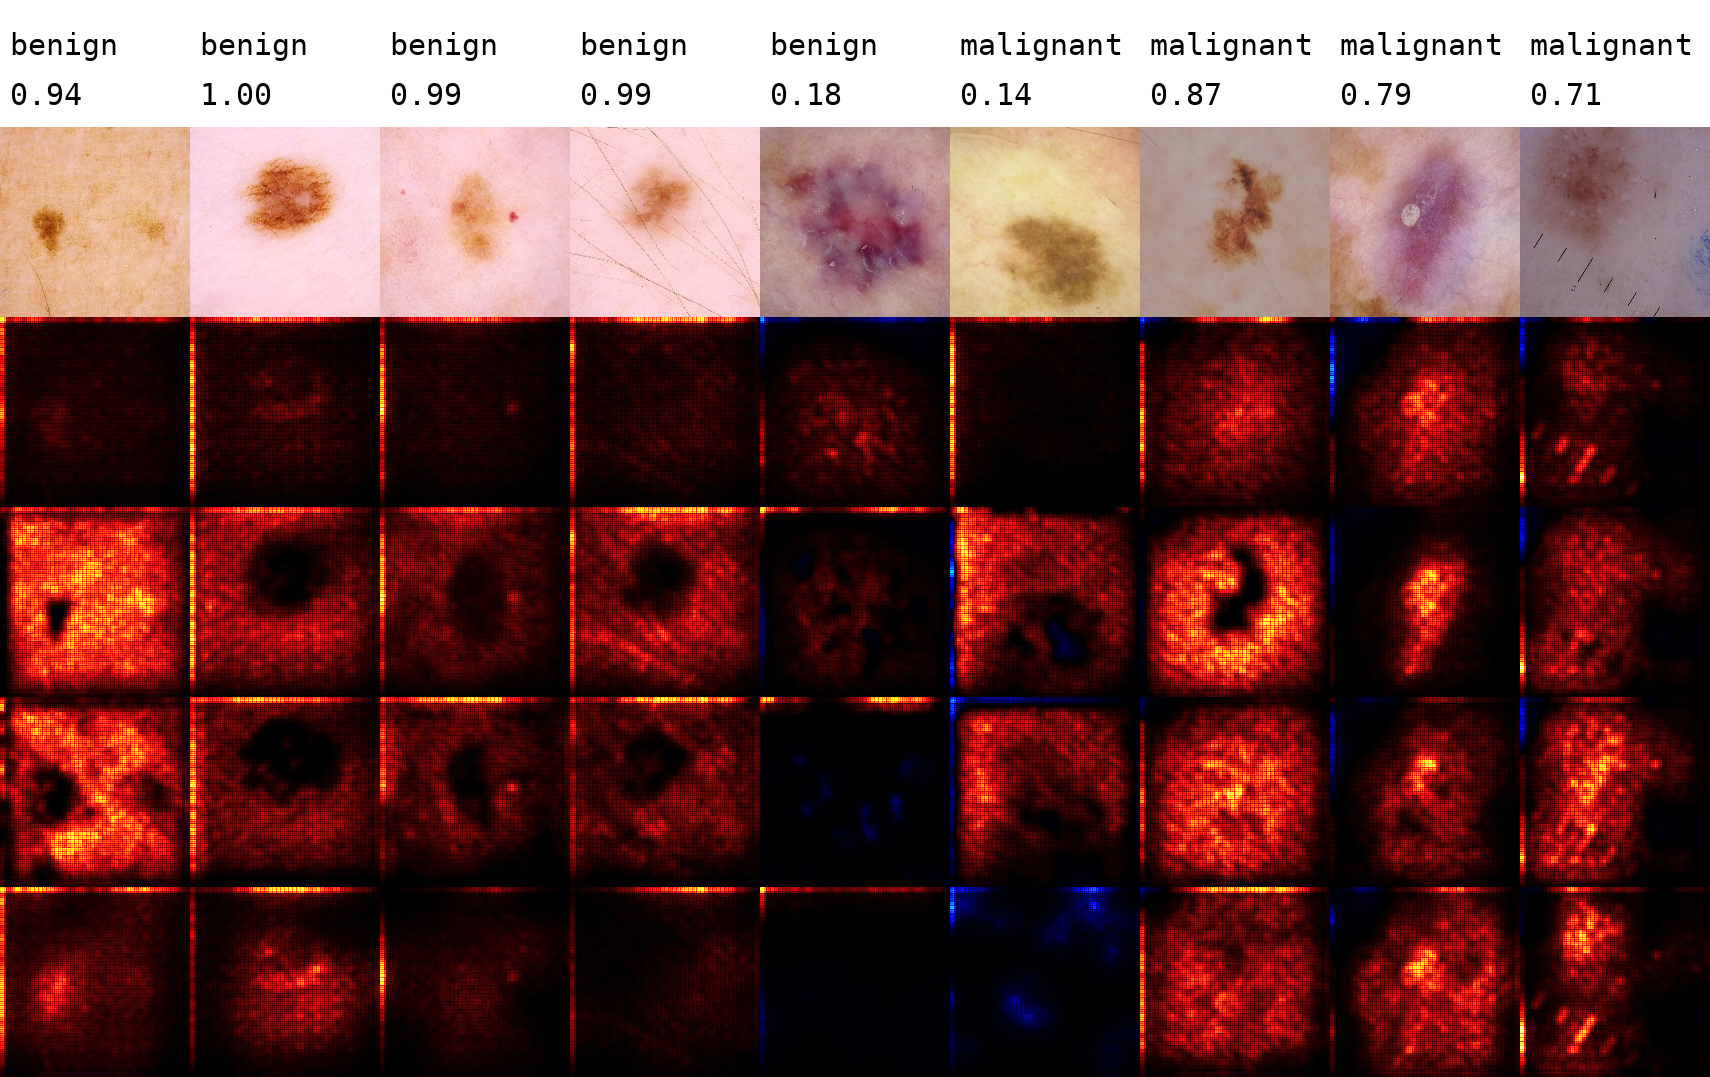
\includegraphics[width=200px]{lrp_crp_melanoma_resnet.png}
    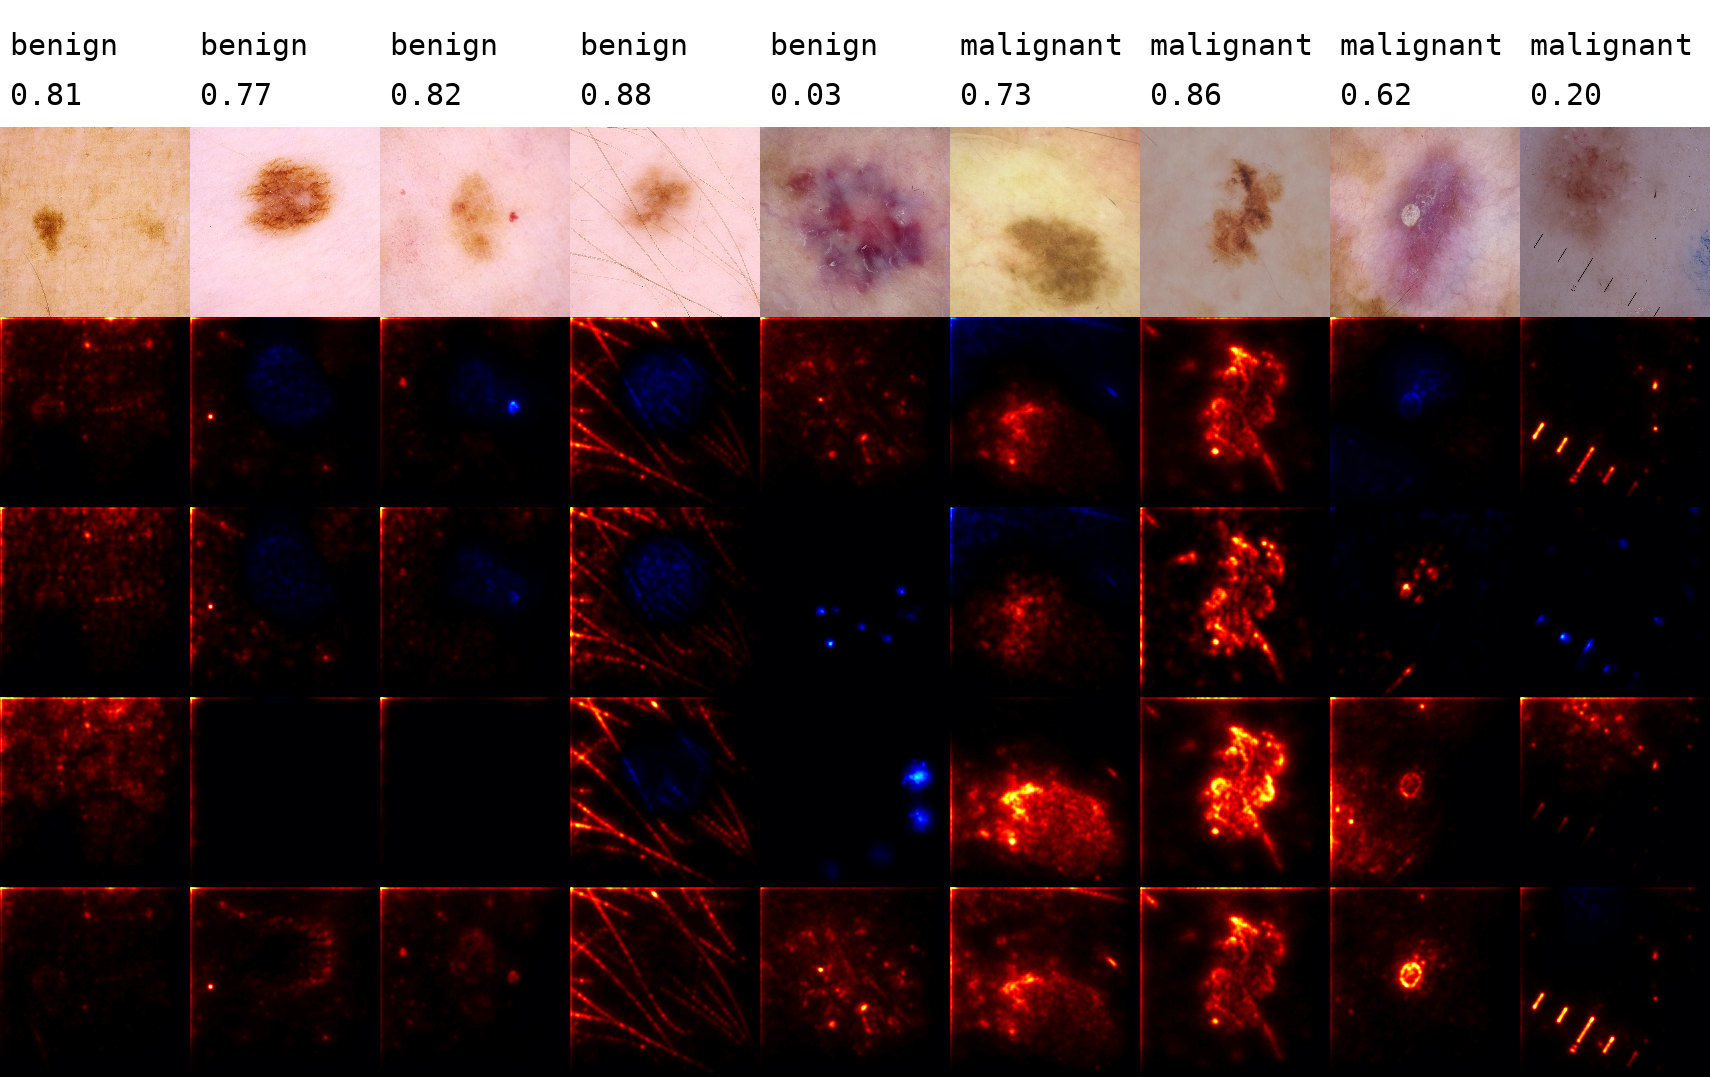
\includegraphics[width=200px]{lrp_crp_melanoma_vgg.png}
    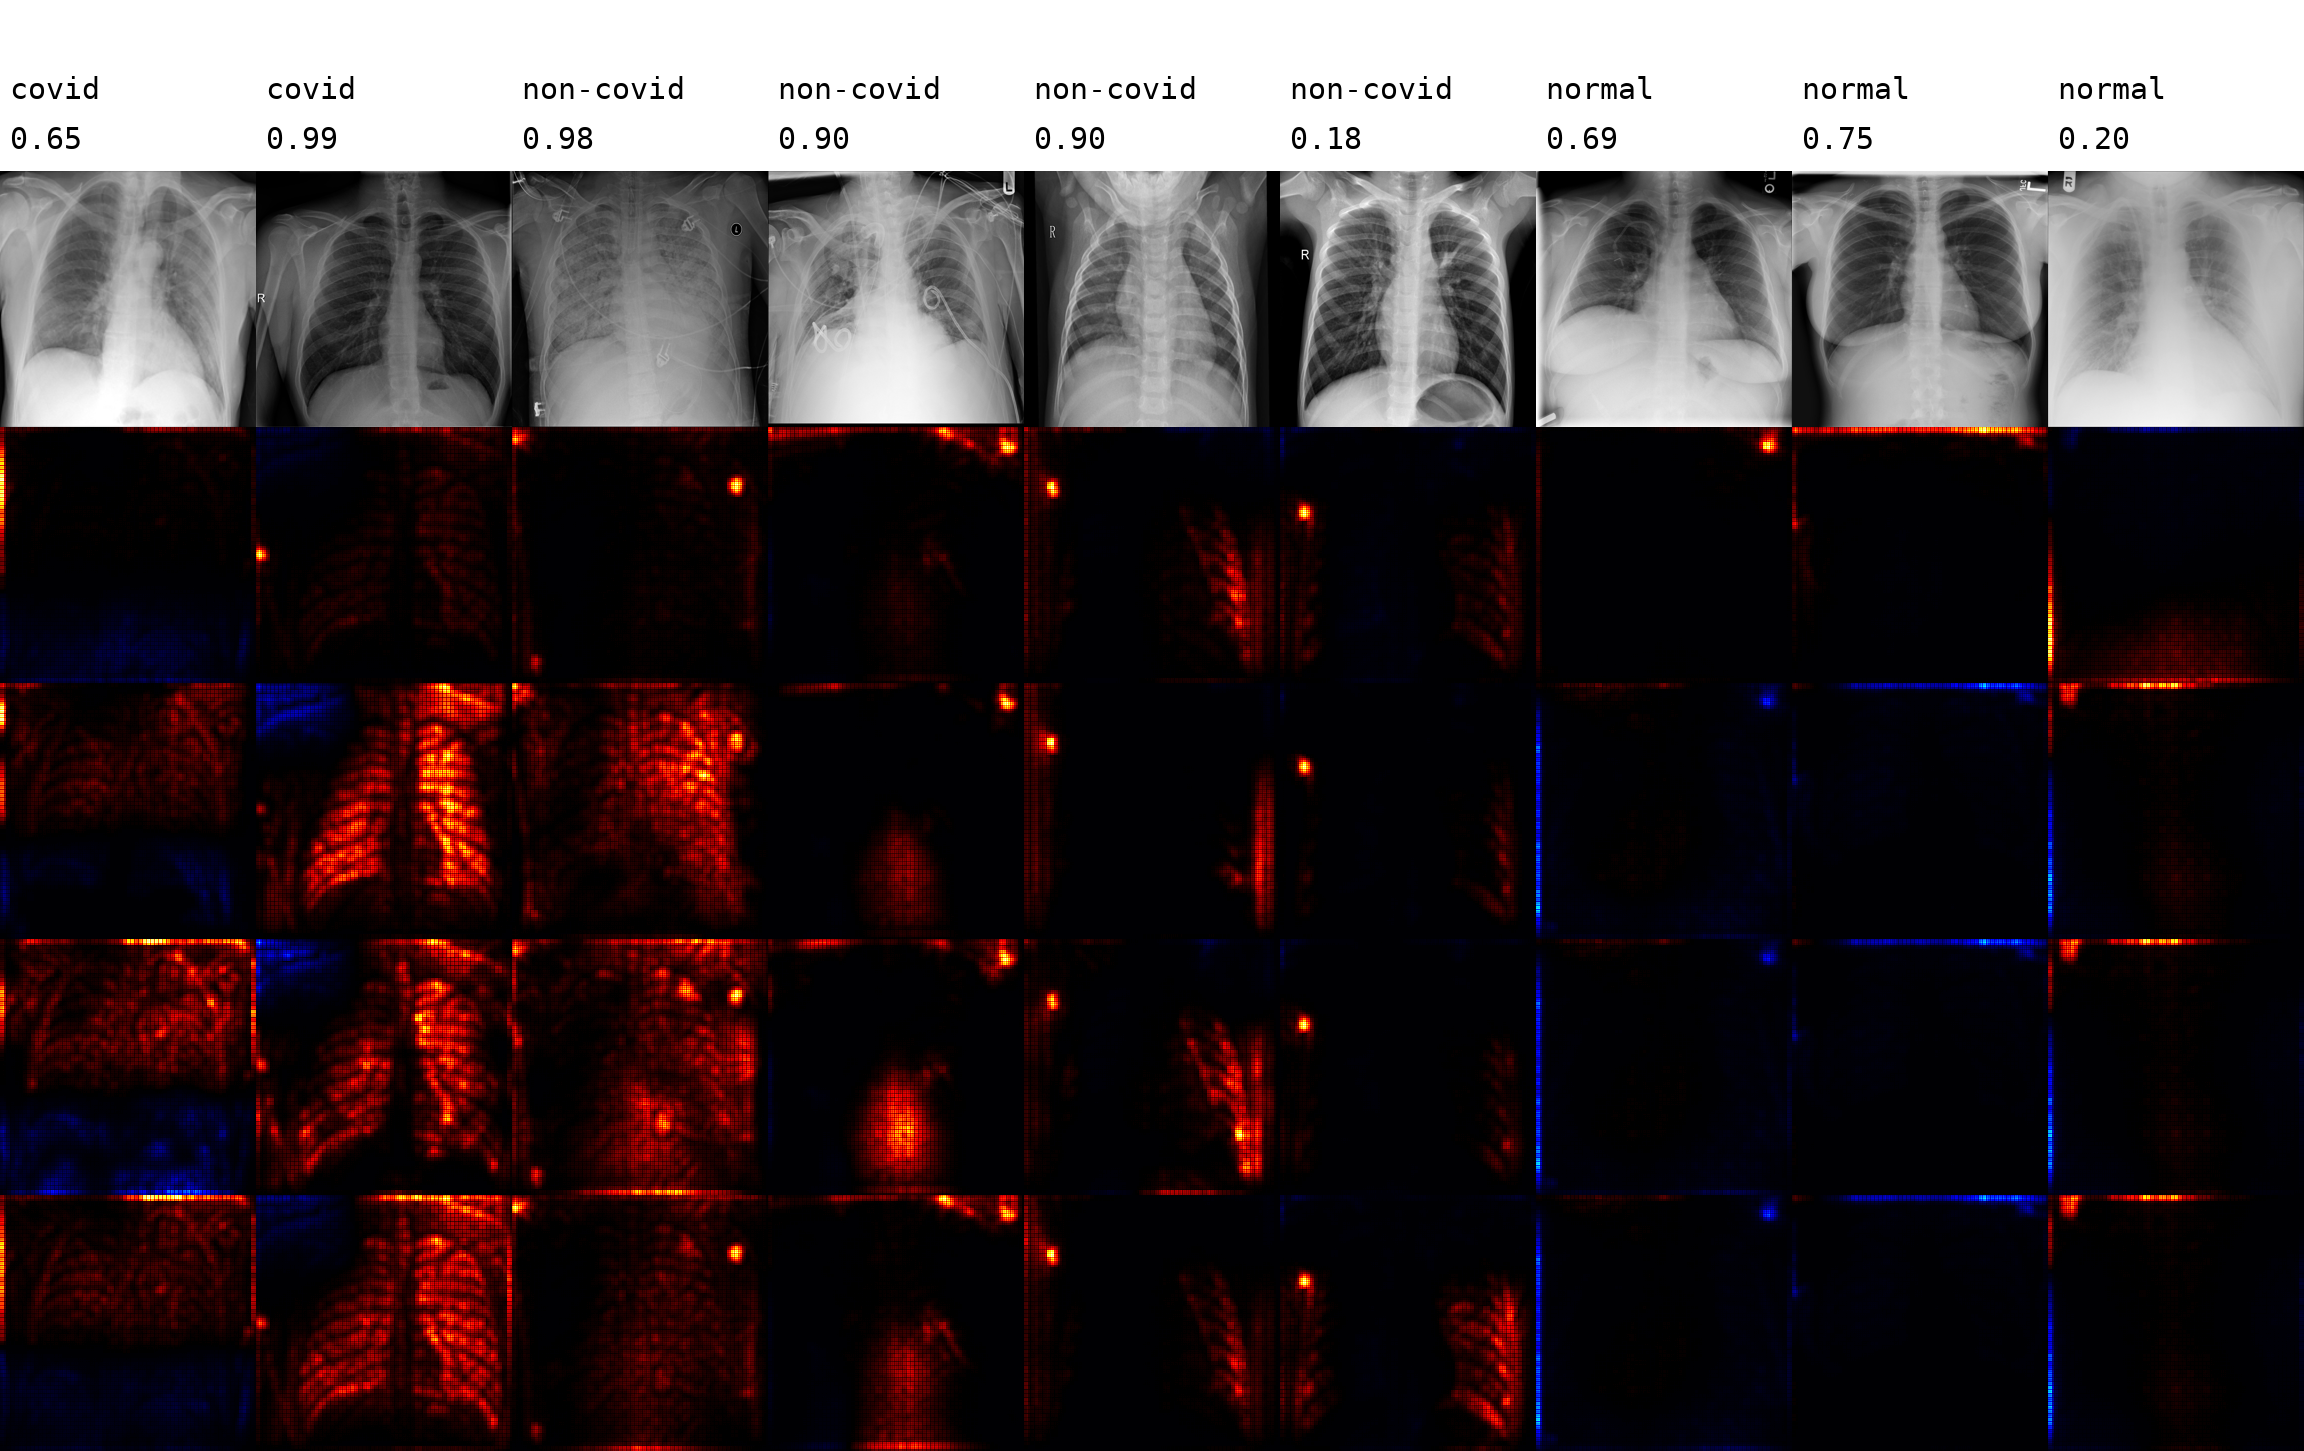
\includegraphics[width=200px]{lrp_crp_covid_resnet.png}
    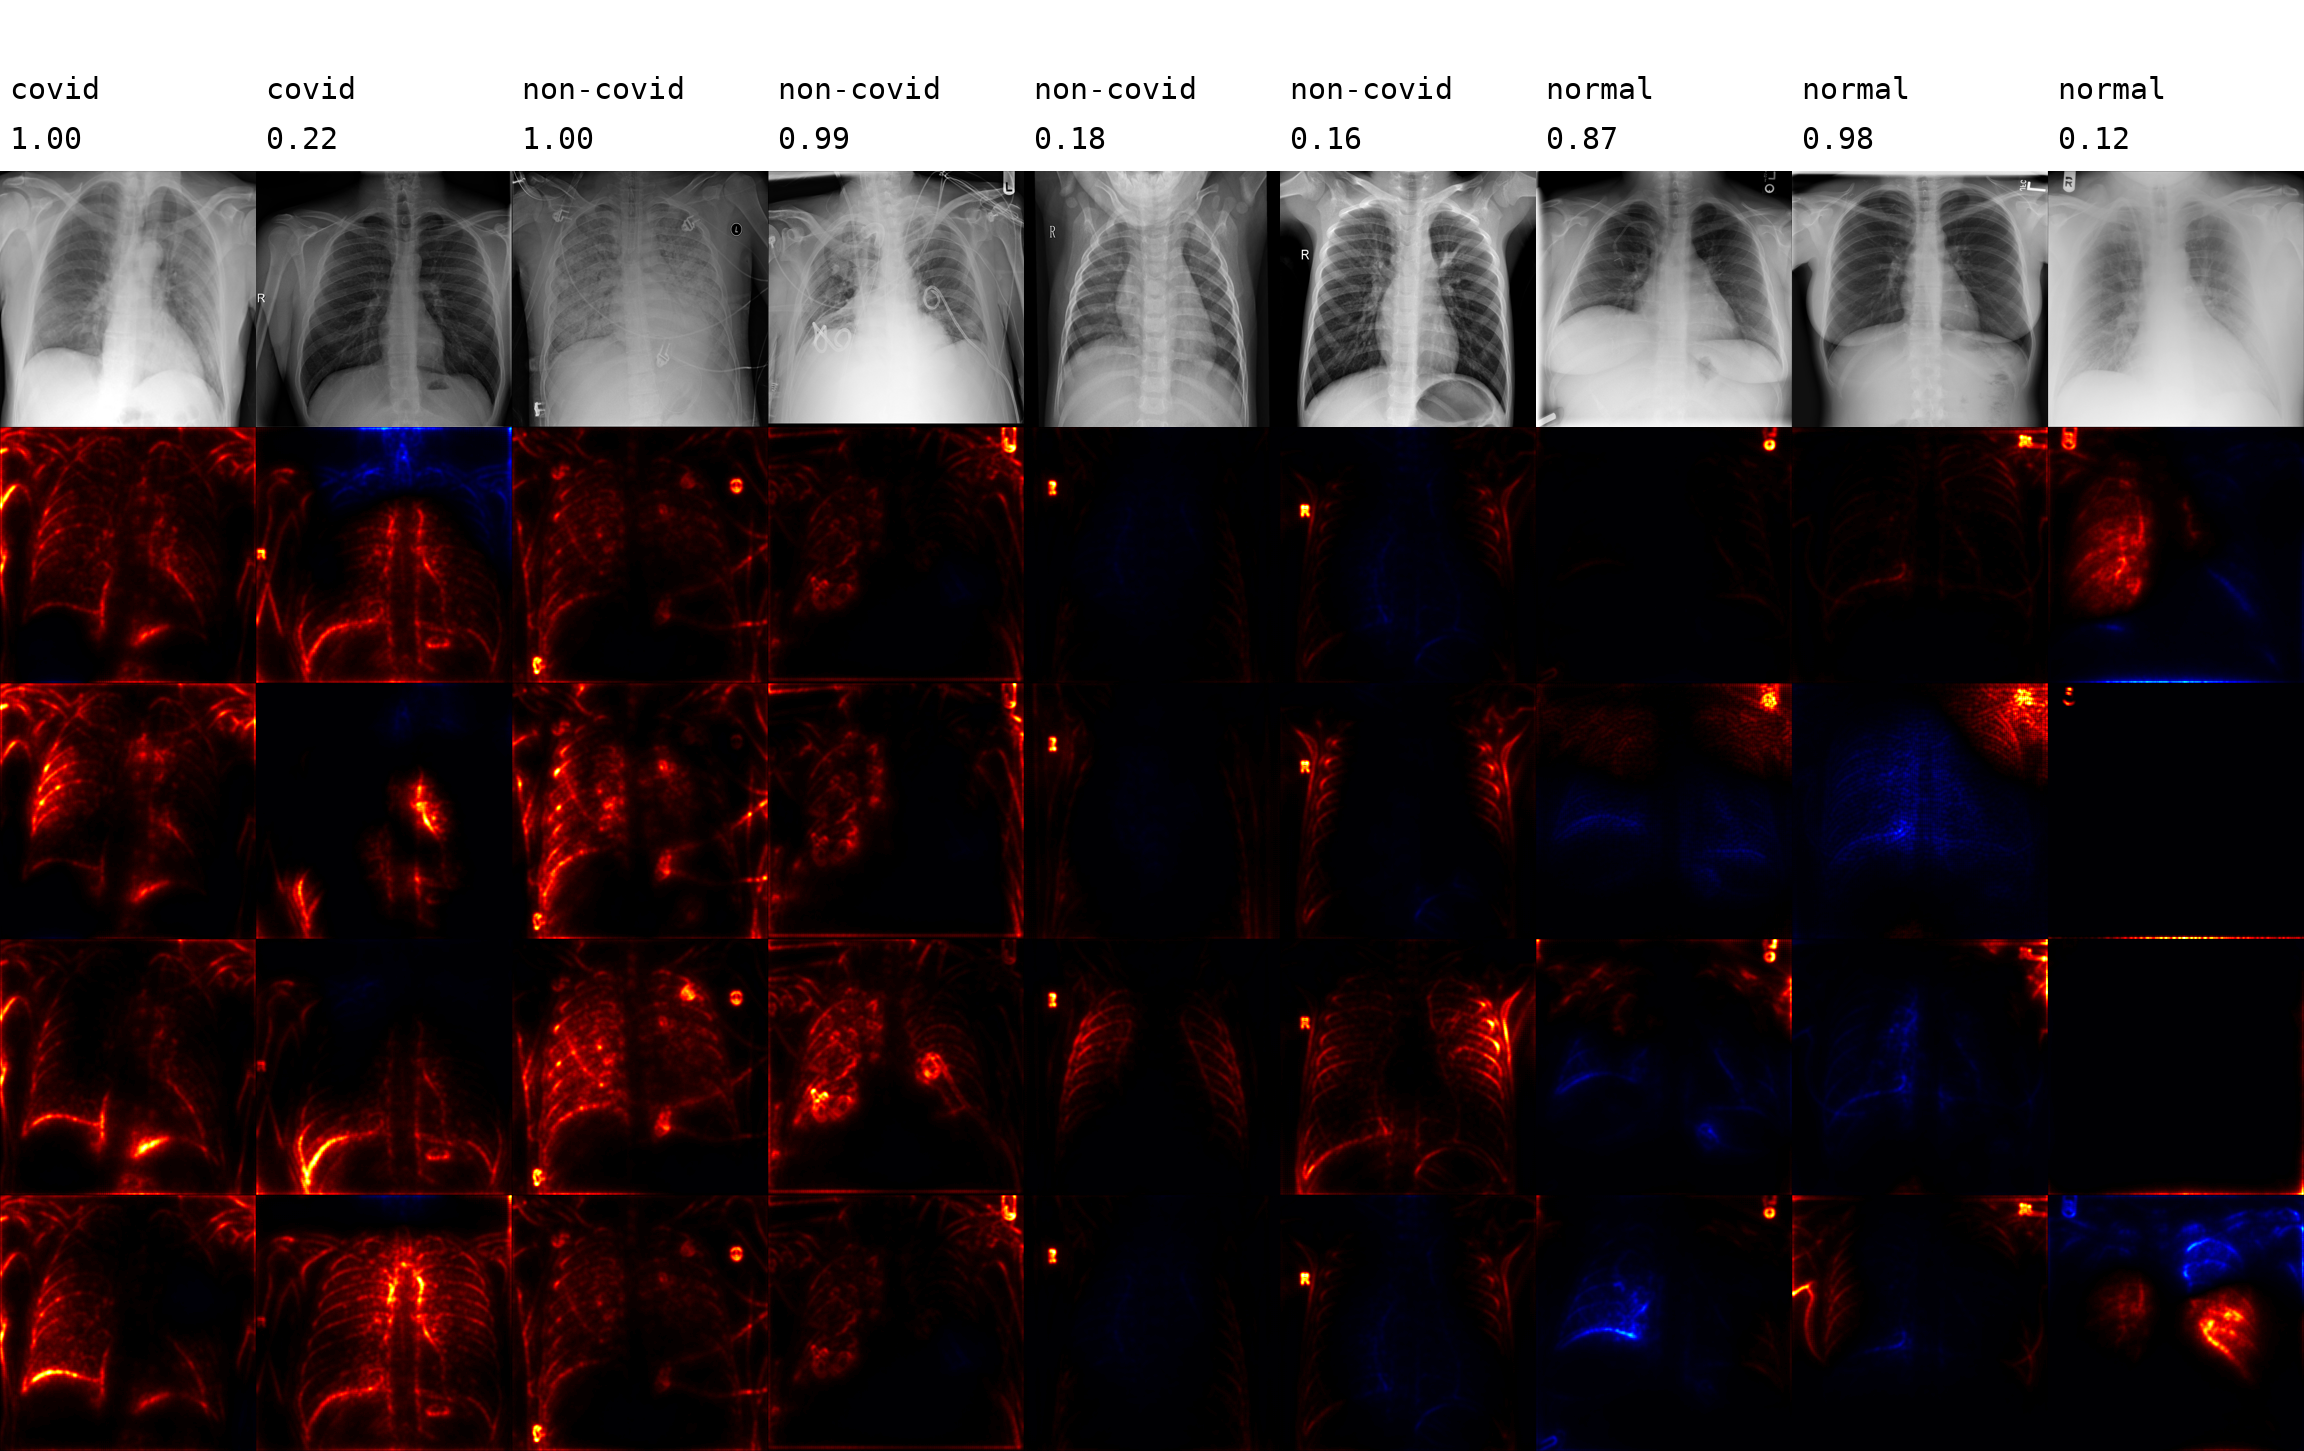
\includegraphics[width=200px]{lrp_crp_covid_vgg.png}
    \caption{
    Melanoma LRP and CRP results (top left: ResNet50, top right: VGG16) and COVID LRP and CRP results (bottom left: ResNet50, bottom right: VGG16).
    On each image the rows are: class name; prediction on the class; input image; LRP explanations with composite EpsilonPlusFlat; 3 CRP explanations conditioned on different layers, from most shallow to deepest.
    More composites for LRP can be viewed in Appendix \ref{appendix:lrp}
    }
    \label{fig:lrp}
\end{figure}

We can observe LRP and CPR explanations for both architectures and datasets in Figure~\ref{fig:lrp}. In general, the LRP in CRP results are quite similar and can lead to related conclusions. The CRP method gives us more explanations and works on different layers which gives us better insights into the models' prediction understanding.

\paragraph{Melanoma Dataset}
We can observe that both models make strong use of features from the skin lesions, the measuring marks, hair, and the border of the image.
Using the border of the image makes sense as in the Melanoma dataset we can observe that benign samples tend to have a light pink background (skin), while malignant are typically darker around the lesion.
Focusing on the measuring marks is probably undesired and may indicate some bias in the dataset.
The presence of hair might be correlated with gender and men are at a higher risk of developing melanoma \citep{rastrelli2014melanoma}, so it makes sense.

% This method confirms all the above conclusions and gives us better insights into the models' prediction understanding. For example, in ResNet the contour is visible in only one of the selected layers - it depends on the color of the skin lesion. This fact was not clear with only LRP. Additionally, in the presence of measuring marks or hair VGG does not really look at other features - looking at different layers gives us more confidence about the interpretations.

% We observe that for some of the layers, the shape of the lesion is being looked at (the same as in the LRP method). It is especially pronounced in the early layers and the observed contours are of a much better quality than in LRP. When the skin lesion is of an atypical color (specifically other than brown) its shape is much more blurry. Hair isn't found to be of particular importance in any of the layers. We can see some color at the borders of images which suggests that it again looks at the skin color. It also looks at the measuring scale but it isn't the dominating concept. Moreover, we can hypothesize that for two examples, which were classified wrong, it was caused by the color of the skin lesion.

% In comparison to ResNet, now we can observe less focus put on the shape of skin lesions in the shallow layers and more in the deeper. The way this can be interpreted is that it's a more 'abstract' kind of shape - so not just the right color but actually 'oh there is something on the skin'. We can observe that changes in the coloring of the skin different from the main object of concern are also found important in some layers, which is great, as their presence is known to be a risk factor for melanoma. Unfortunately, the model seems to put much focus on hair and scale for growth measurement in comparison to ResNet.


\paragraph{COVID Dataset}
The models focus on three main aspects: left/right X-ray lead markers, the overall lung area, and the border of the image.

The roentgen left/right markers are used by radiologists to label which lung is which one and are visible as single letters on the images. The explanations suggest that both methods find those letters important. This is highly undesired - a possible explanation for this bias is that our dataset could be unequally distributed between clinics or laboratories that use different markers.

The overall lung area is where we expect the model to focus. Here the VGG16 explanations again look more convincing. The most interesting cases are the ones where we can see both negative and positive attribution from different parts of the image. For example, in the right-most column, we can see a wrongly classified healthy lung (0.12 prediction from this class). The left lung (the right one in real life according to the marker) looks healthy and has a positive attribution. The other one is smaller, less visible, and has a negative impact on the score, which is reasonable.

The border of the image is the least desired feature here. The ResNet50 model focuses quite intensely on it. It might mean that there are some more biases in the data and perhaps some other augmentations should be used.

Additionally, the explanations for the 'normal' lungs are the least visible. This might make sense because of our asymmetrical  dataset - there might be no characteristics of healthy lungs, just some features of sick ones.

% It is clearly visible that ResNet extracts some features about the lungs, ribs, and heart, all of which might be relevant for diagnosing a disorder. For VGG we can find that the model focuses on features that are a bit different.

% Additionally, while for the 'normal' labeled samples, there isn't much attribution apart from the side of the image, it might make sense - because there probably aren't many characteristics of healthy lungs, so that just can mean 'nothing out of ordinary'. It is clearly visible that ResNet extracts some features about the lungs, ribs, and heart, all of which might be relevant for diagnosing a disorder. For VGG we can find that the model focuses on features that are a bit different.


\paragraph{Checker pattern}
\begin{figure}[t]
    \centering
    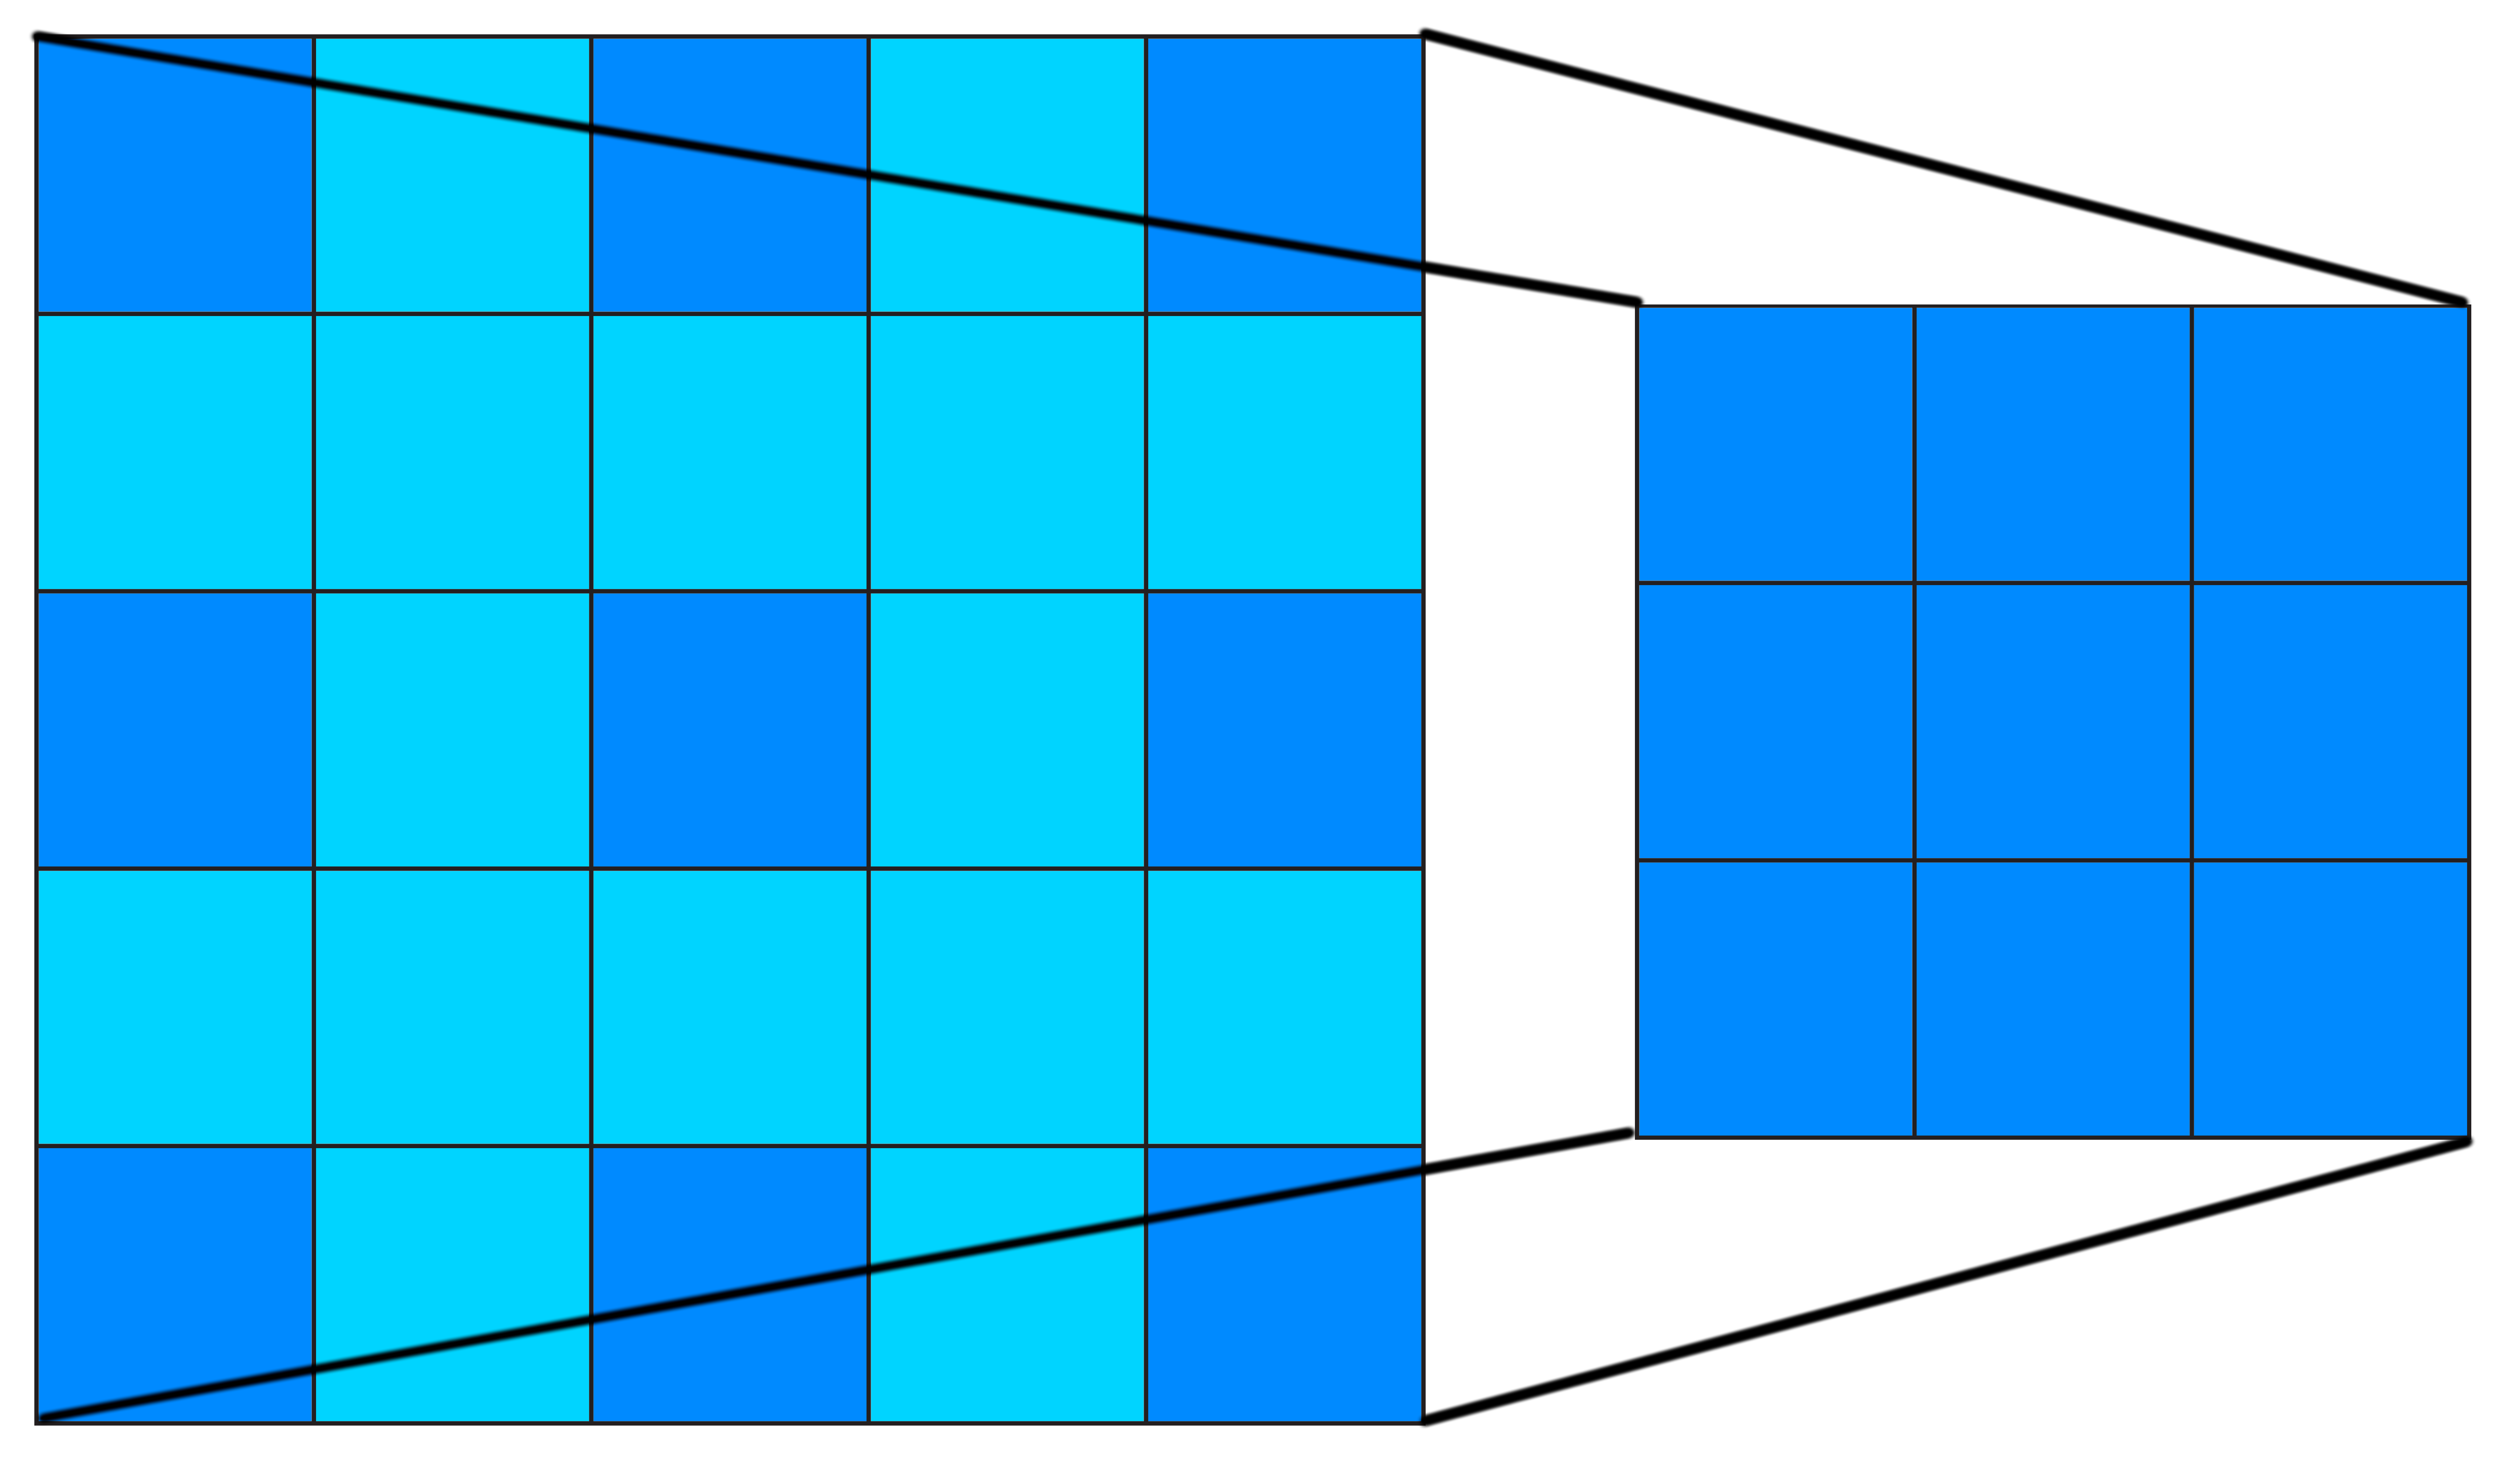
\includegraphics[height=50px]{conv.png} \quad
    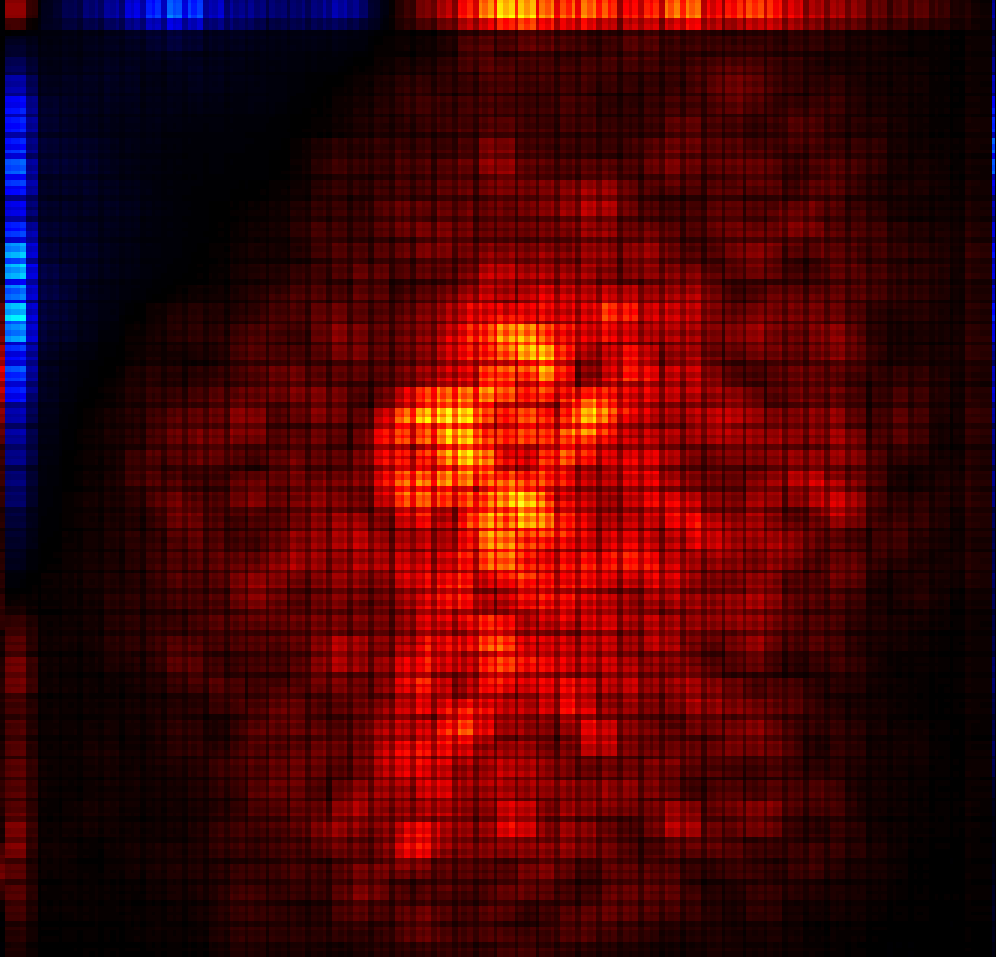
\includegraphics[height=50px]{short_checker_resnet.png} \quad
    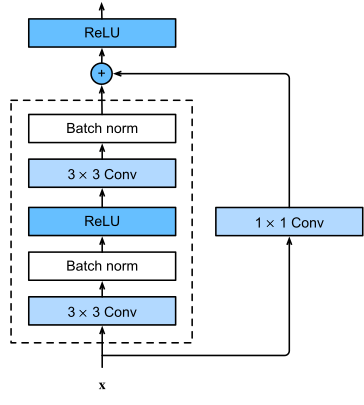
\includegraphics[height=50px]{resnet_block.png}
    \caption{1x1 convolution layer with stride 2 (left), zoomed ResNet50 LRP explanation (middle), ResNet block (right).}
    \label{fig:resnet_residual}
\end{figure}
There is one worrisome characteristic visible in the ResNet explanations - a visible checker pattern. 
This phenomenon is caused by the residual connections present in the ResNet architecture (Figure \ref{fig:resnet_residual}).
Residual blocks that scale down the image use a 1x1 convolution with a stride equal to 2.
This results in the checker pattern visible in LRP and CRP explanations as the signal is much stronger in the pixels that were used in residual connections.

\paragraph{ResNet vs VGG}
The LRP results are better for the VGG architecture on both datasets - the VGG manages to better highlight lung or skin changes shapes. Additionally, VGG's explanations have more often parts with both positive and negative attribution on the same image, which is helpful in interpreting those results. The differences come from the architectures - ResNet cannot be naturally divided into layers as opposed to VGG with no residual blocks. In CRP both models give different, interesting results. In Melanoma ResNet does not extract the hair and measuring marks, which might be better. The borders of skin lesions are more clearly visible. In the COVID dataset, ResNet and VGG look at quite different features. Specialist knowledge is required to verify which features are more important.

% In LRP (Figure \ref{fig:lrp}) we can see that explanations for VGG architecture are better.
% They do not consist of any checker pattern as opposed to ResNet.
% In the case of the COVID dataset, the VGG manages to highlight lung shapes as opposed to ResNet.
% On the Melanoma dataset, the explanations are also better in the case of the VGG architecture. The shapes of the skin lesion are much more visible. Additionally, VGG's explanations have more often parts with both positive and negative attribution on the same image.
% It seems that VGG just better suits the LRP method.
% Its architecture can be naturally divided into layers as opposed to ResNet which has residual blocks.

\paragraph{Robustness}
\begin{figure}[t]
    \centering
    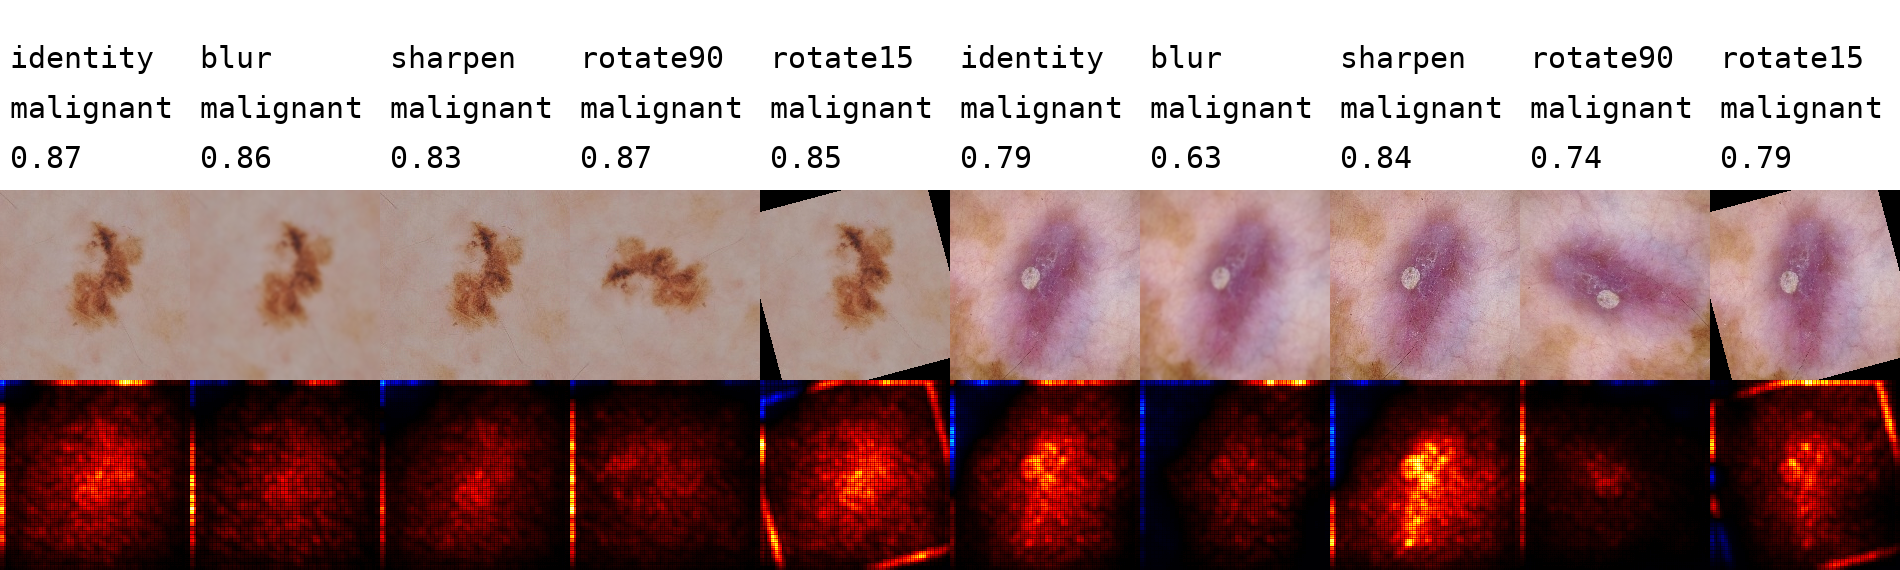
\includegraphics[width=200px]{short_tta_melanoma_resnet.png}
    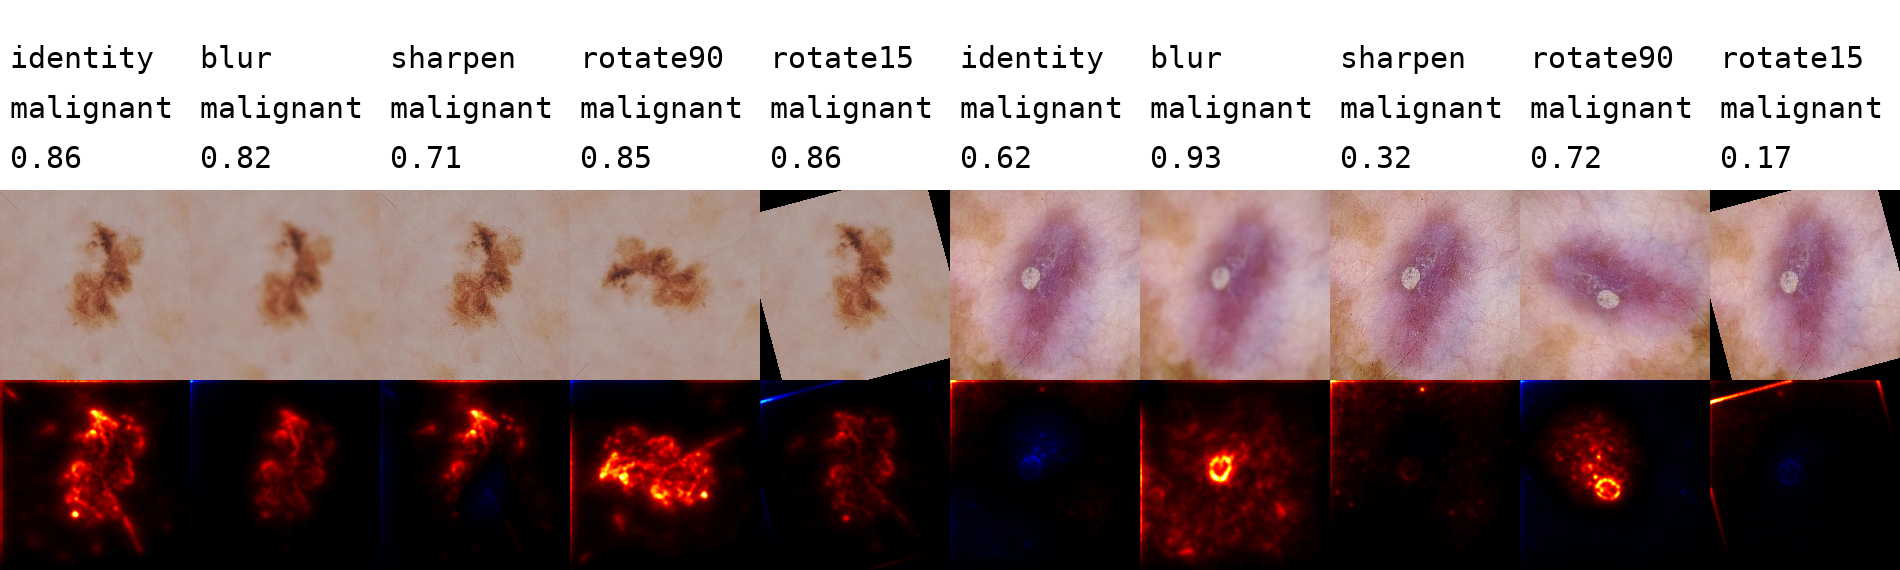
\includegraphics[width=200px]{short_tta_melanoma_vgg.png}
    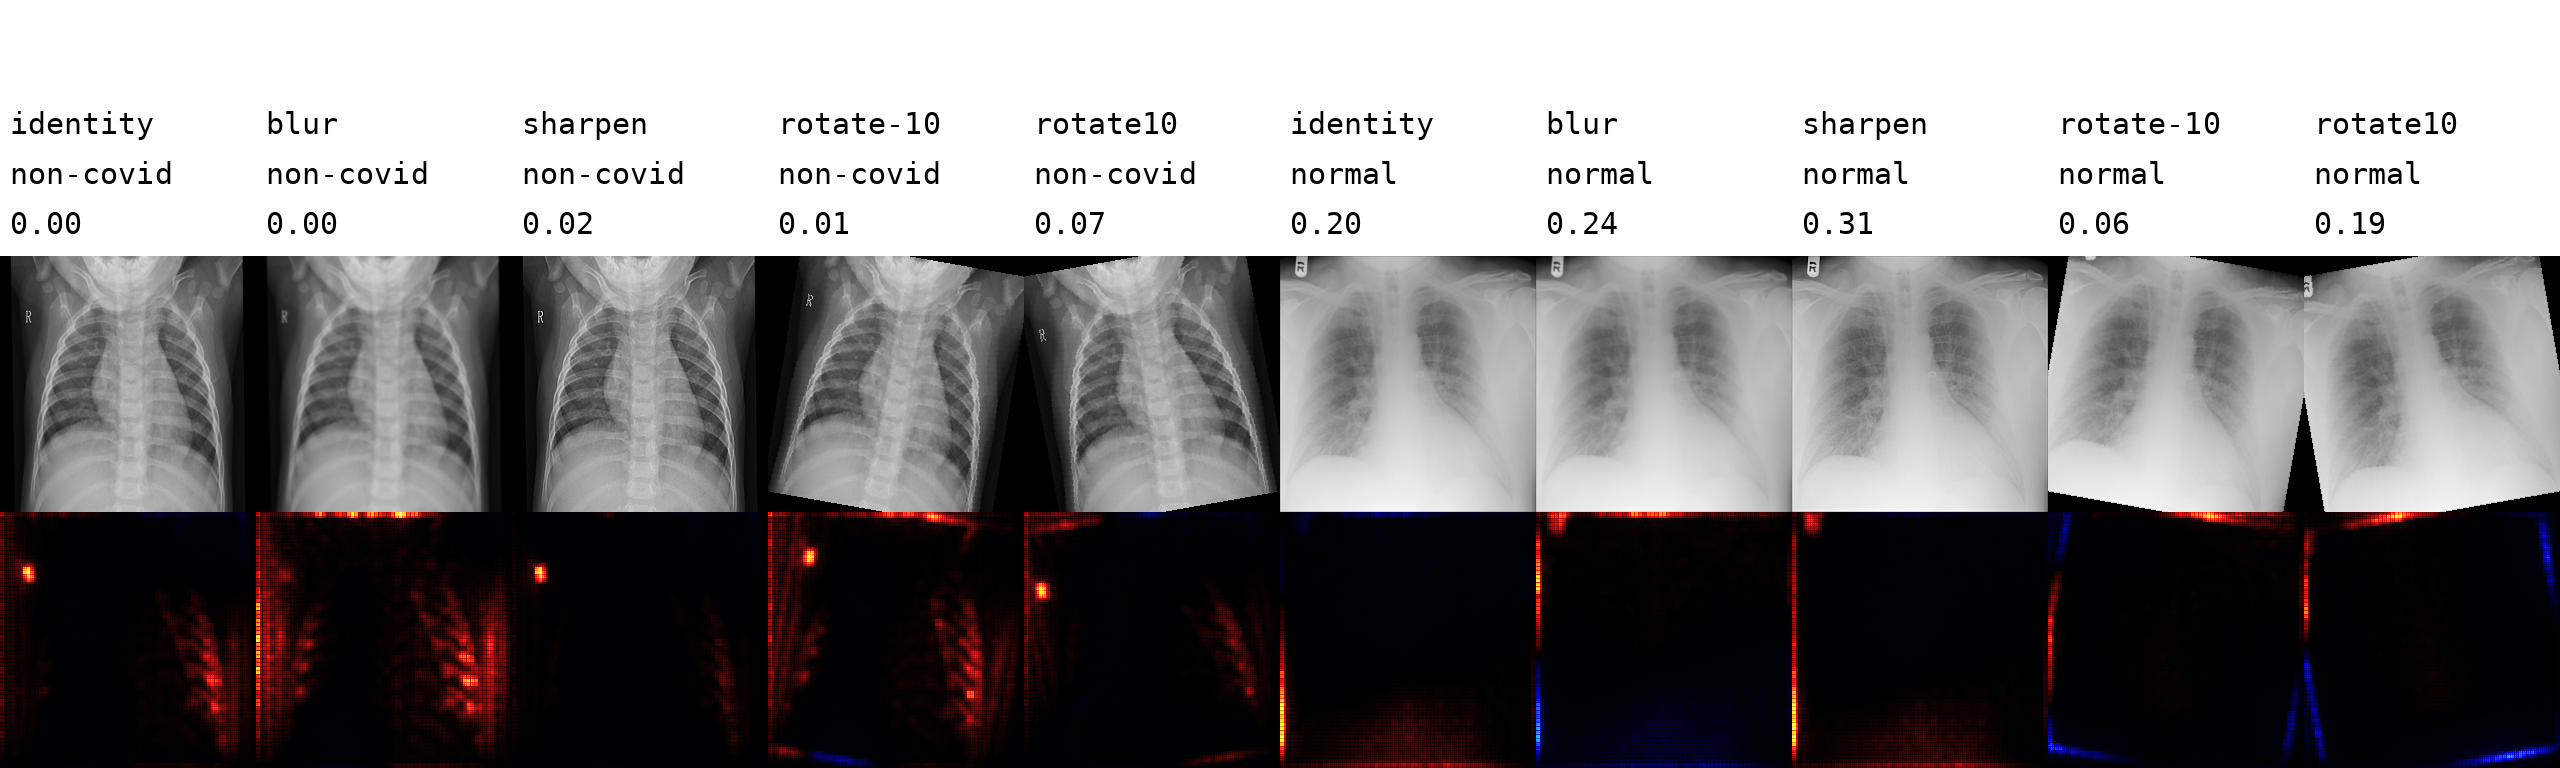
\includegraphics[width=200px]{short_tta_covid_resnet.png}
    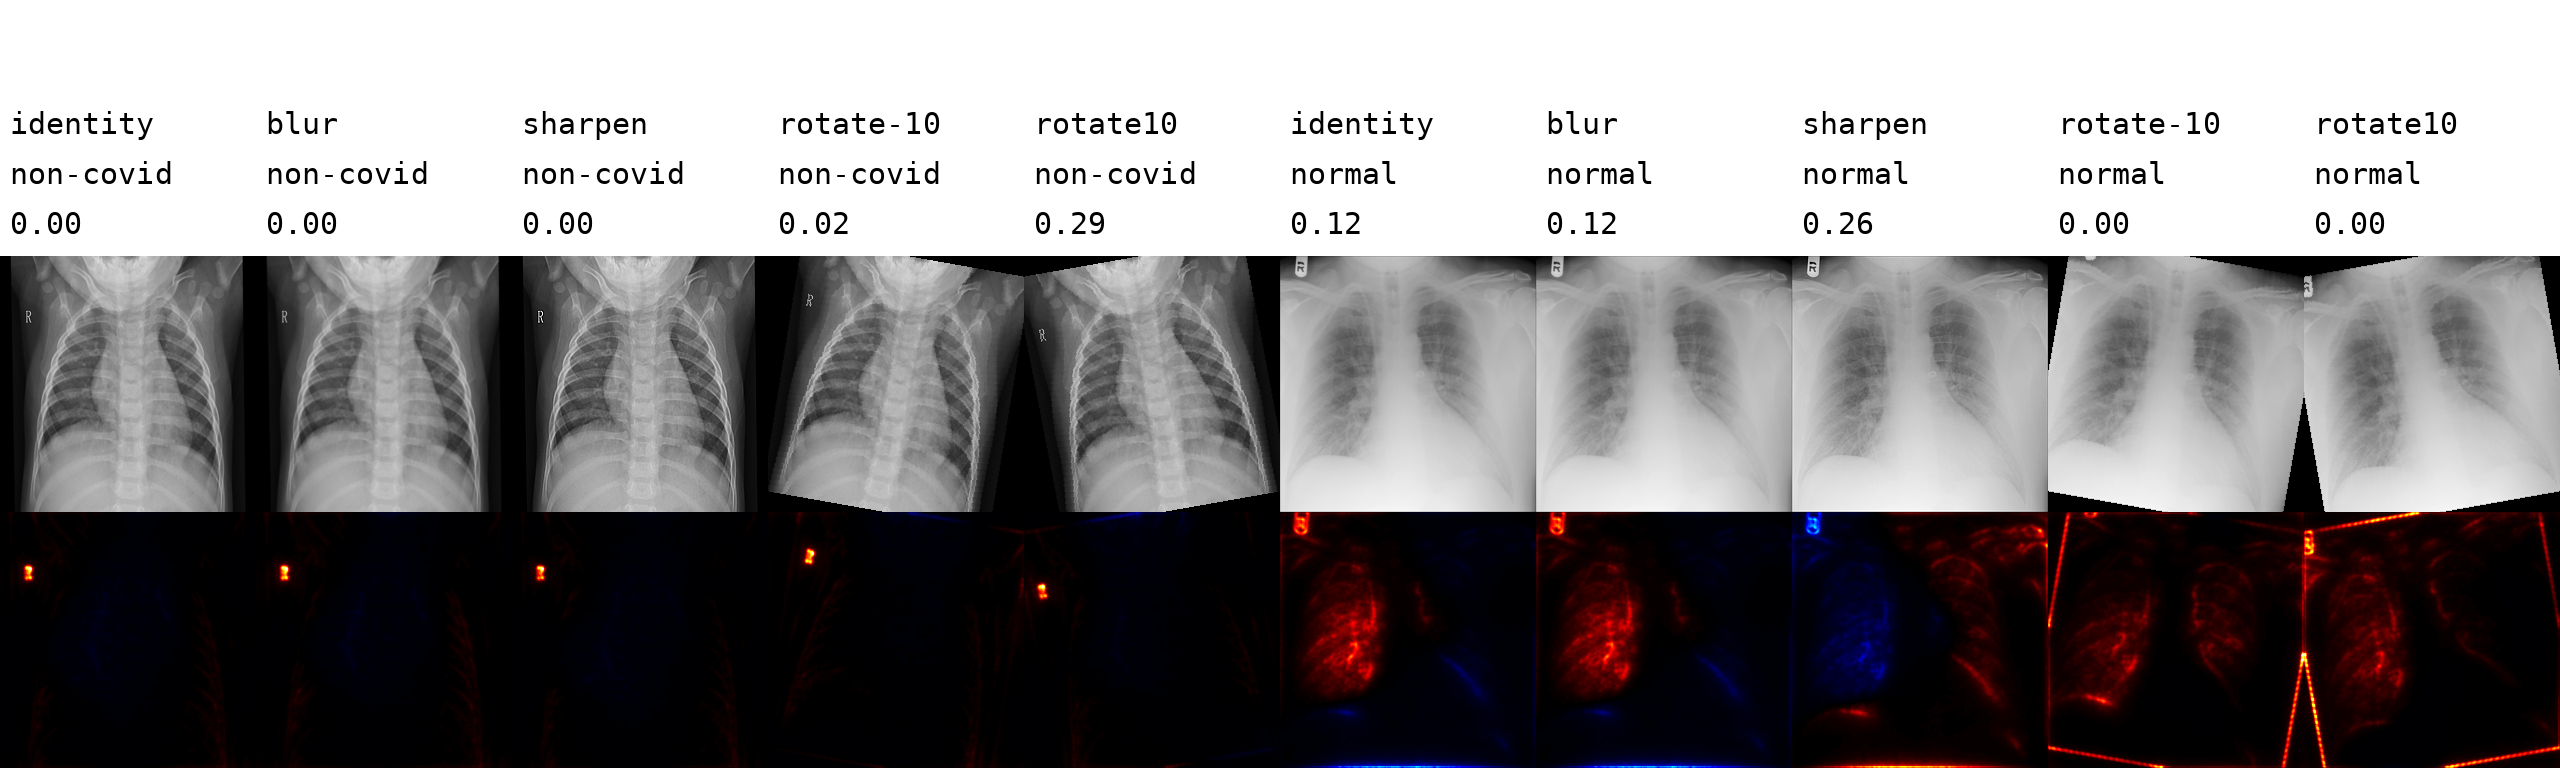
\includegraphics[width=200px]{short_tta_covid_vgg.png}
    \caption{
    Results for LRP after input augmentation.
    Melanoma LRP results (top left: ResNet50, top right: VGG16) and COVID LRP results (bottom left: ResNet50, bottom right: VGG16).
    On each image, the rows are augmentation name, class name, prediction on the class, input image, and LRP explanations with composite EpsilonPlusFlat.
    More composites can be viewed in Appendix \ref{appendix:lrp}
    }
    \label{fig:lrp_tta}
\end{figure}

To evaluate the robustness of the LRP we compared the visualizations after applying different augmentations to the input image. We have tested blur, sharpen, and rotations (Figure \ref{fig:lrp_tta}).
We can observe that the explanations change drastically in the case of the VGG architecture.
On the COVID dataset, the positive and negative heatmap can even swap places.
On the Melanoma dataset, we can observe that the same skin lesion once attributed positively and once negatively depending on augmentations.
ResNet results are more consistent, although they are still quite different.
We can conclude that LRP evaluations for CNNs are not robust.
Most likely, this is due to the known CNNs' vulnerability to augmentations and adversarial attacks \citep{pgd_madry}.

% \begin{figure}[t]
%     \centering
%     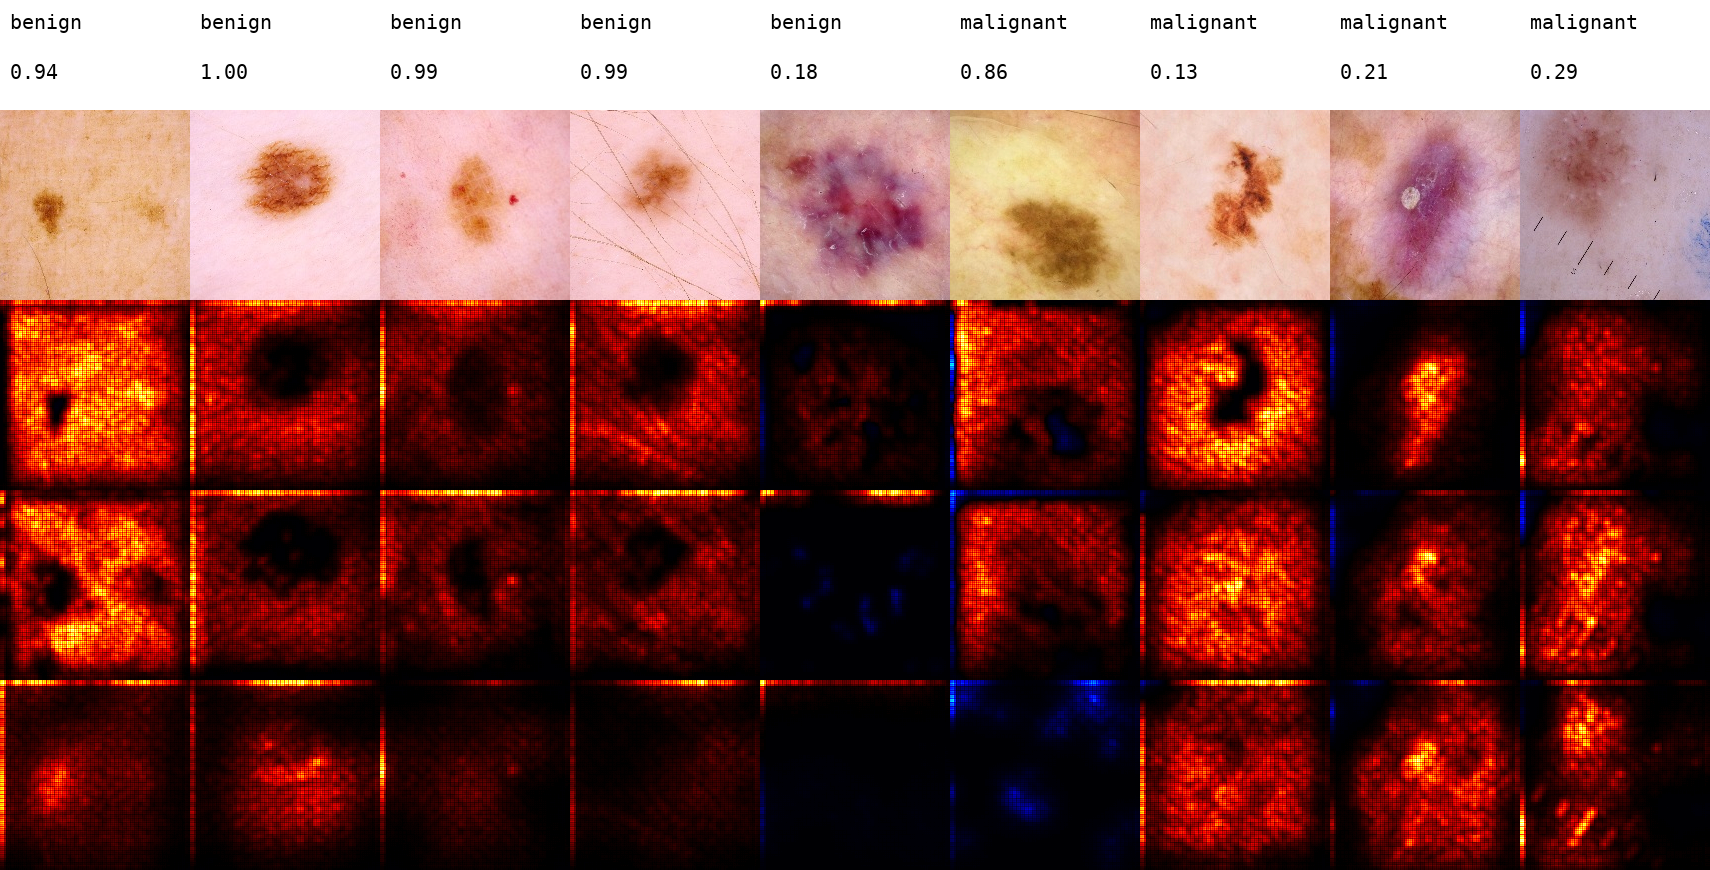
\includegraphics[width=200px]{crp_melanoma_resnet.png}
%     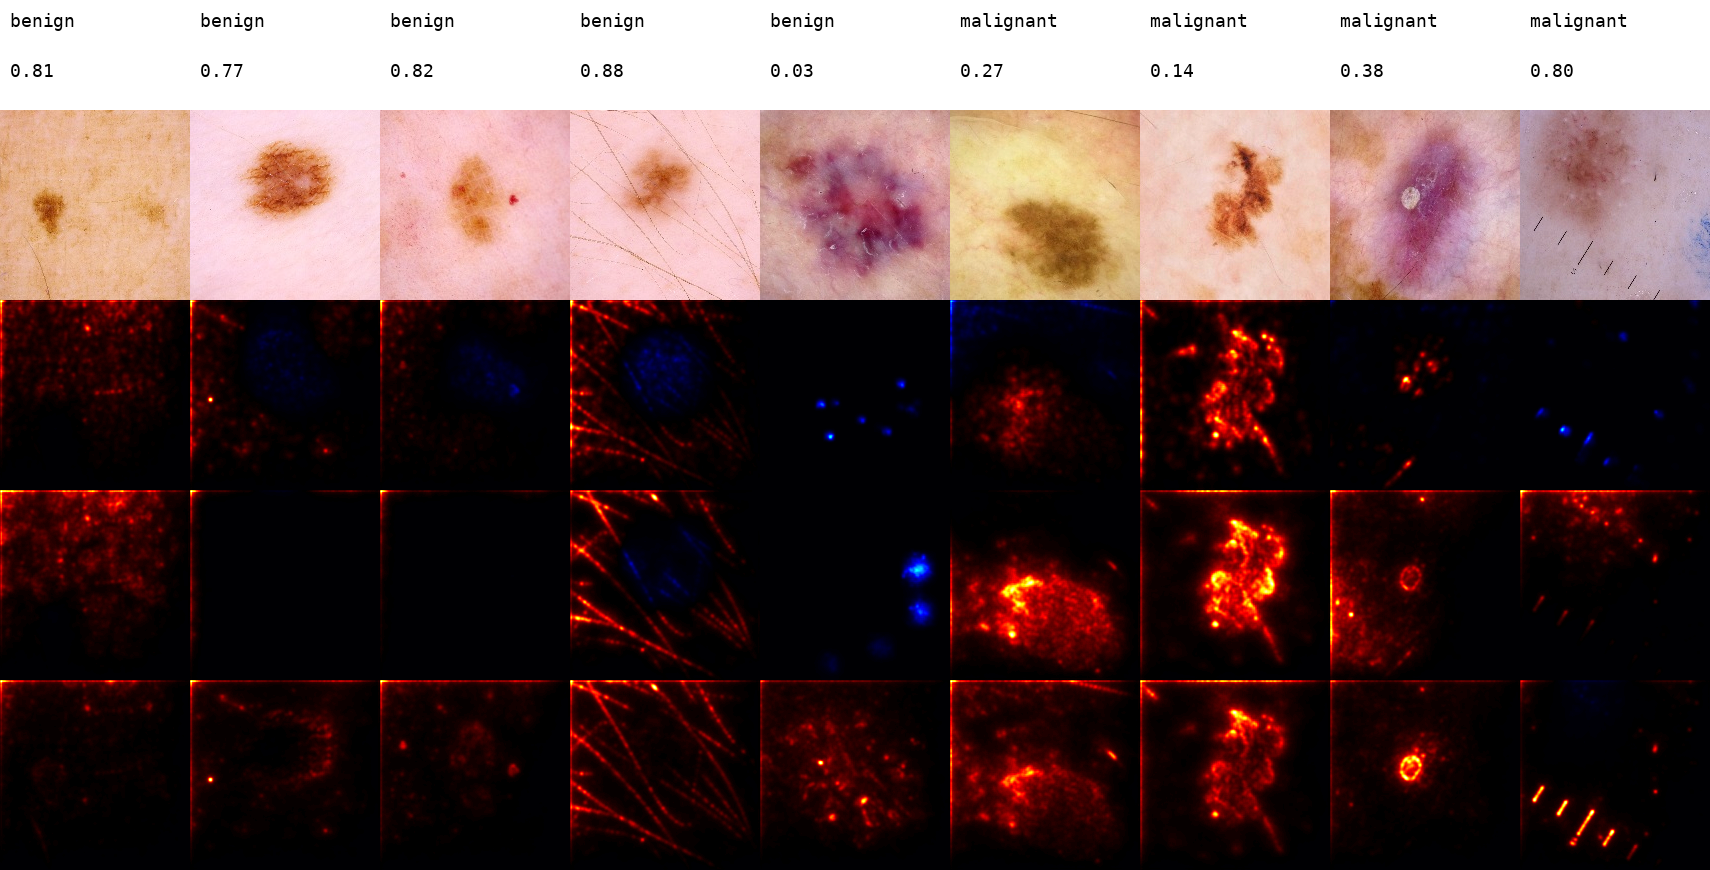
\includegraphics[width=200px]{crp_melanoma_vgg.png}
%     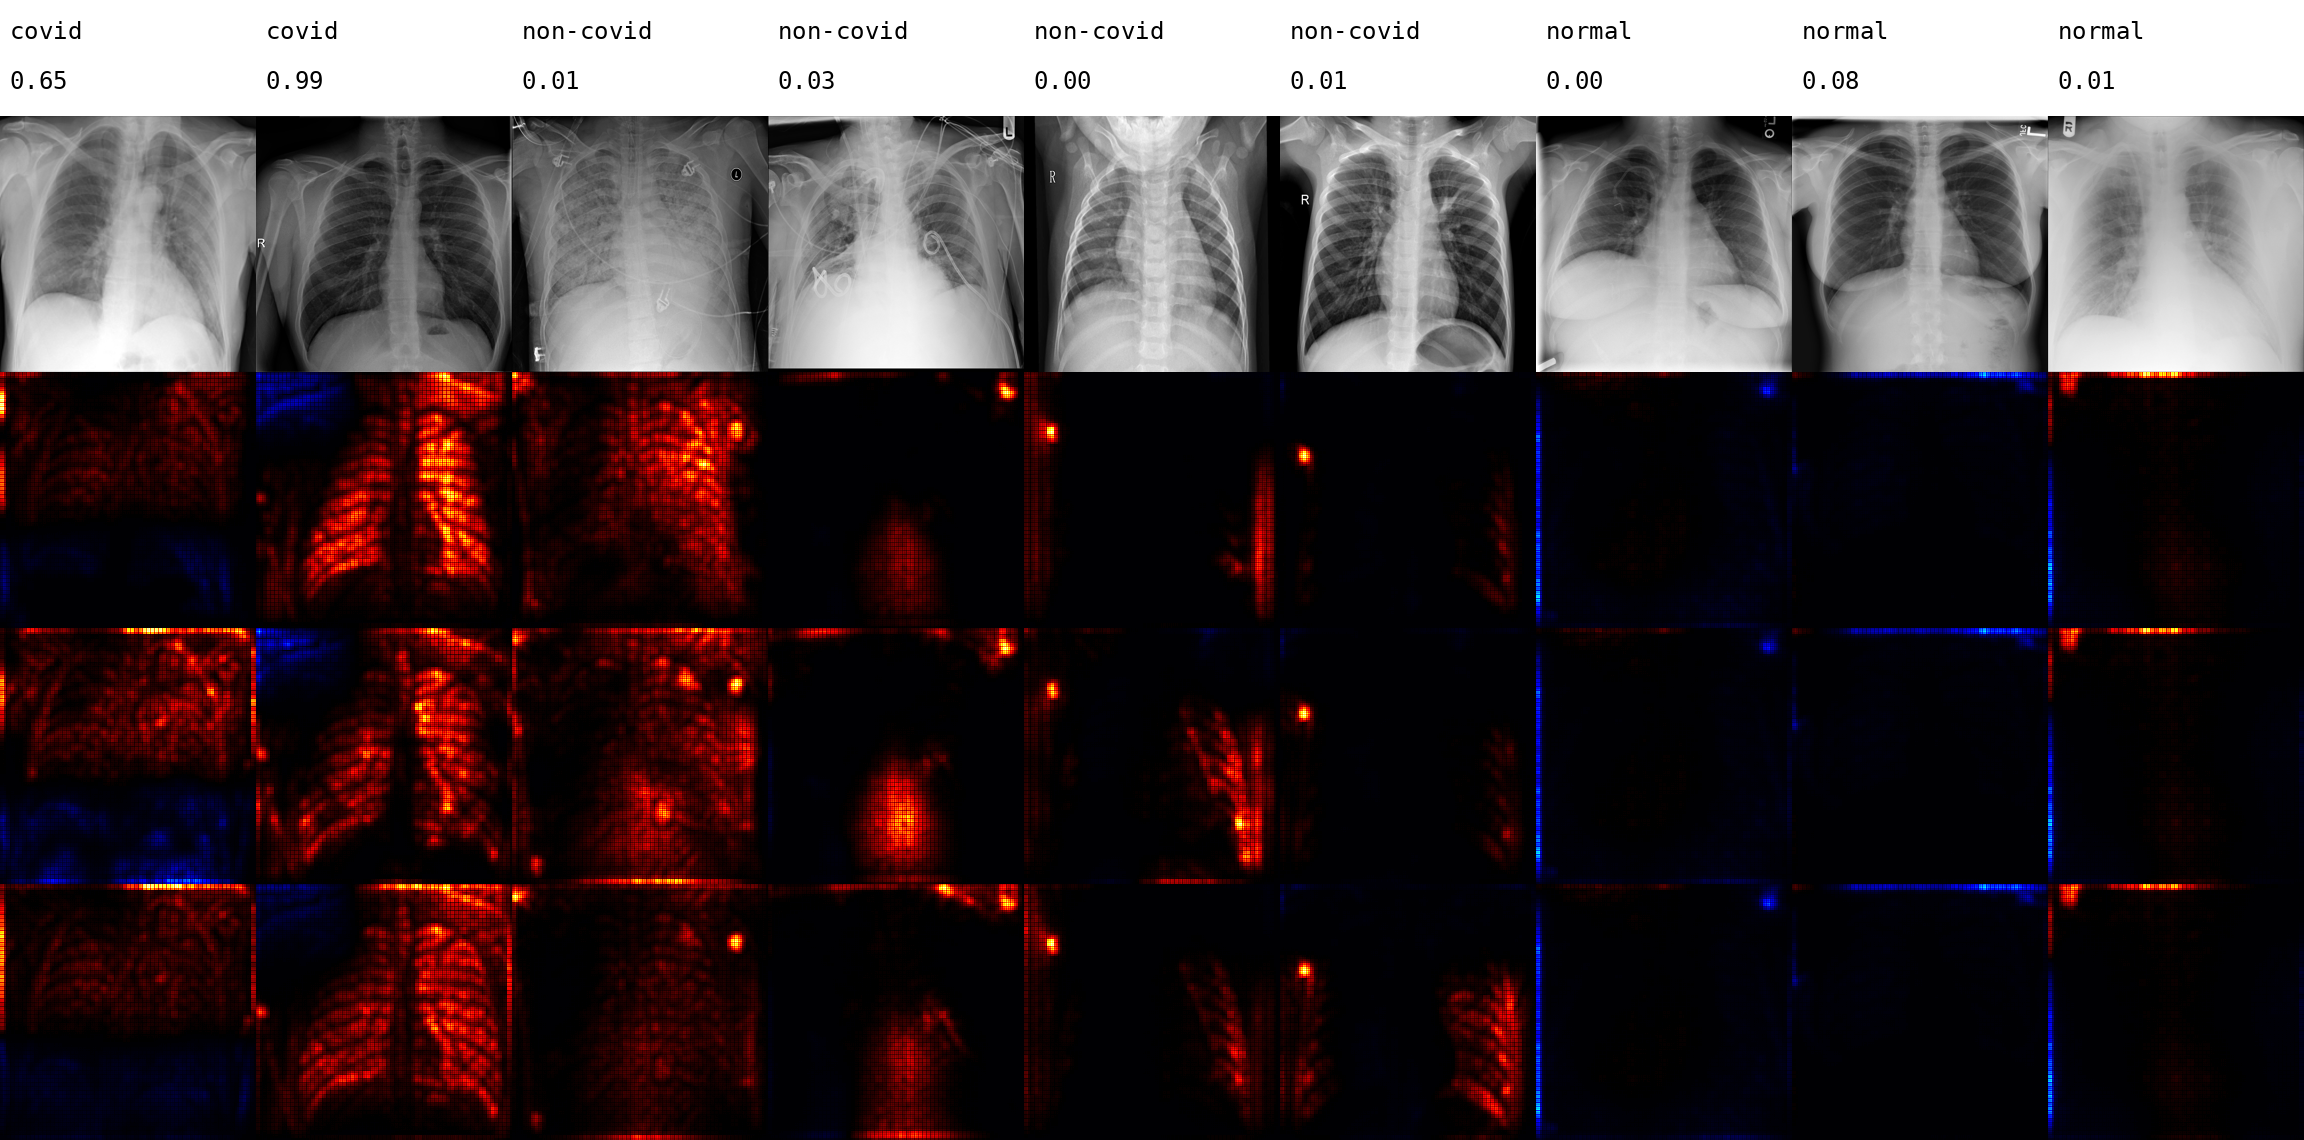
\includegraphics[width=200px]{crp_covid_resnet.png}
%     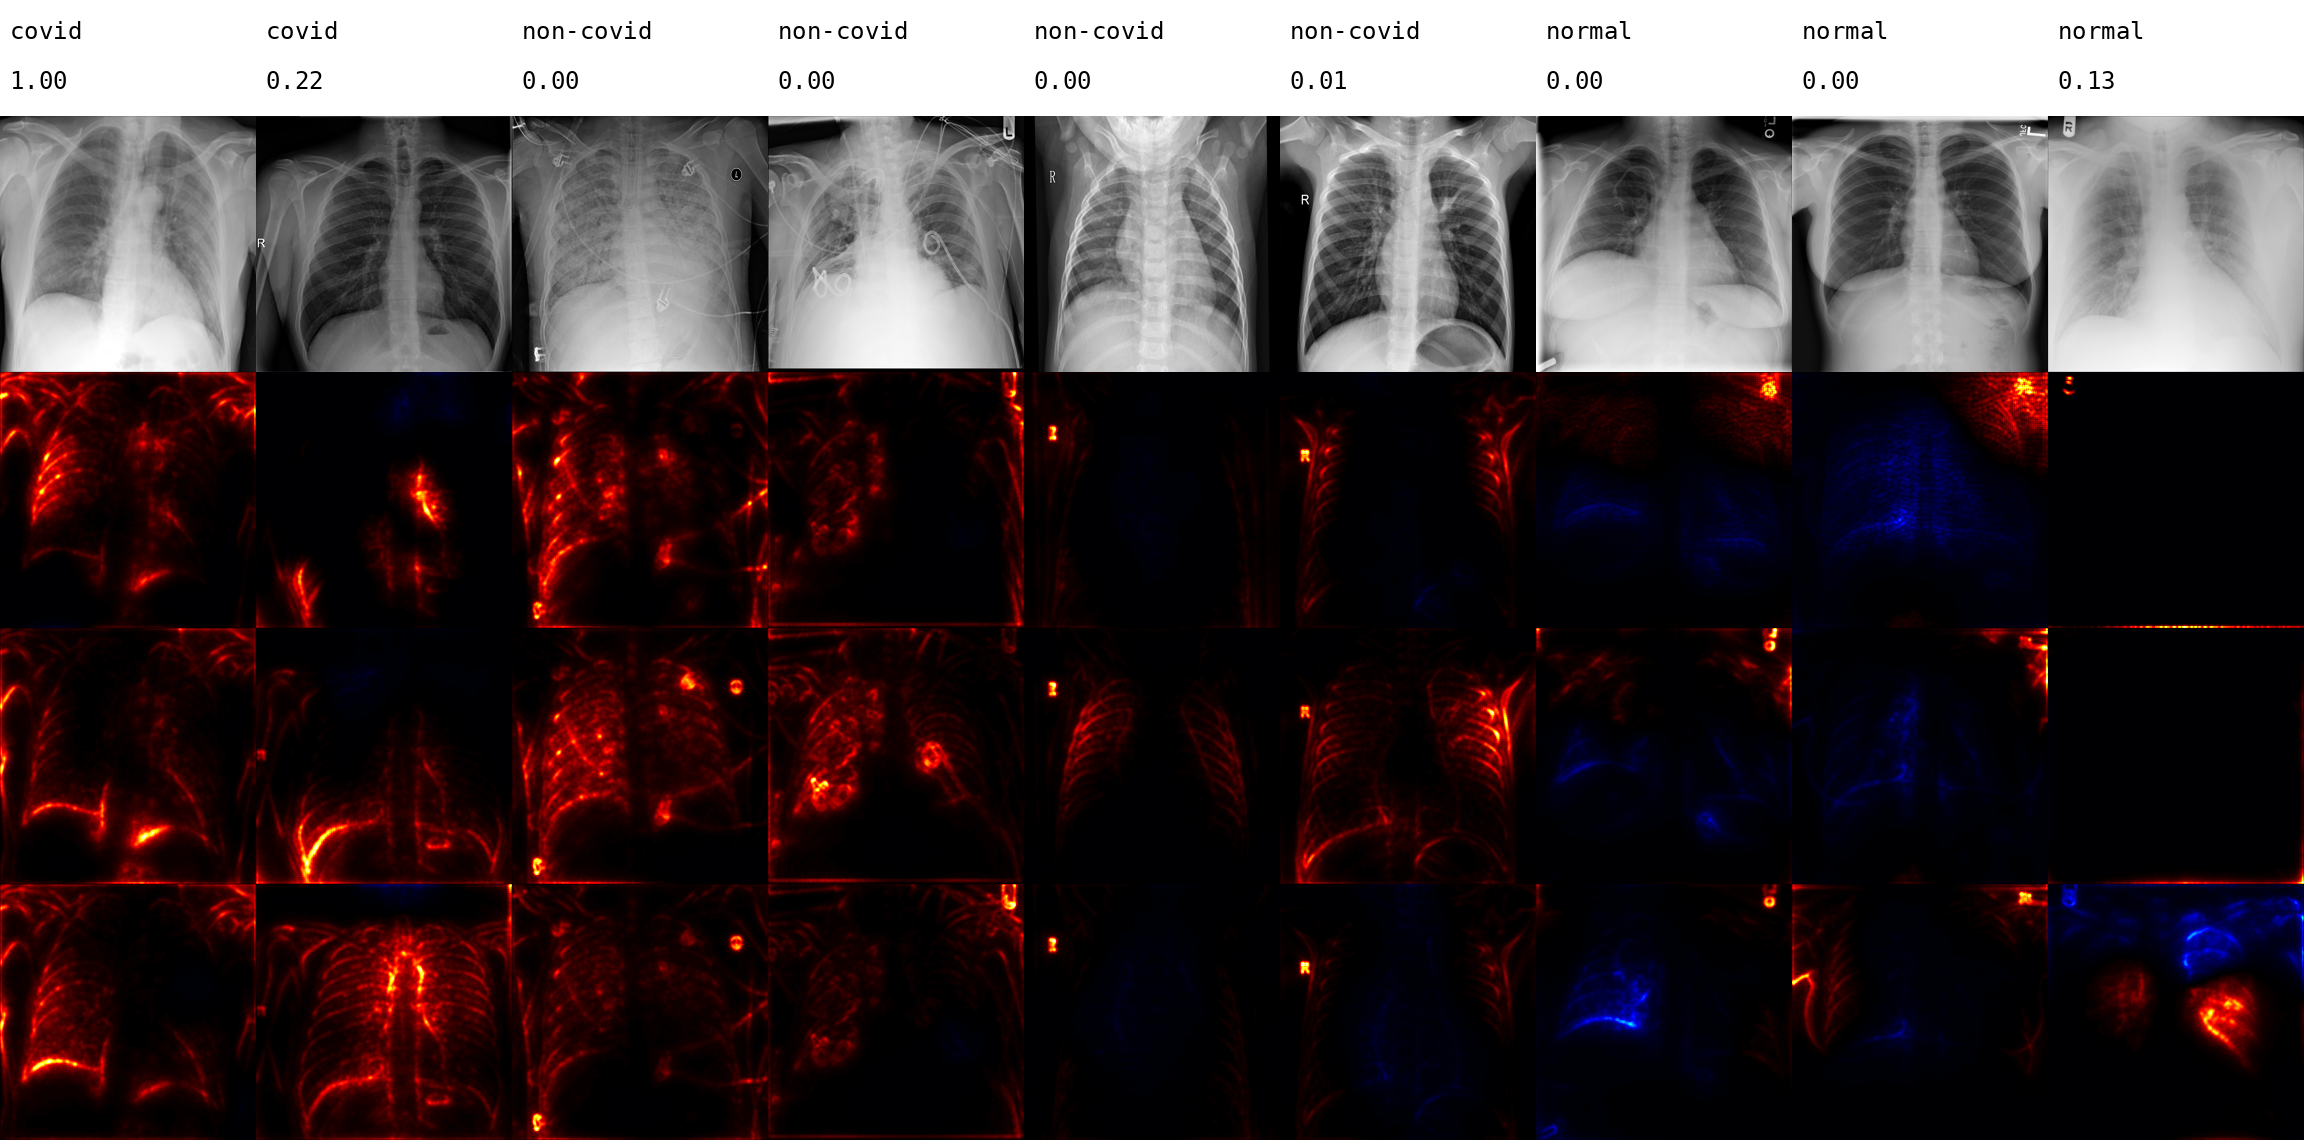
\includegraphics[width=200px]{crp_covid_vgg.png}
%     \caption{
%     Results for CRP method.
%     Melanoma CRP results (top left: resnet, top right: VGG) and COVID CRP results (bottom left: resnet, bottom right: VGG).
%     Conditioned on different layers, from most shallow to deepest.
%     }
%     \label{fig:lrp_tta}
% \end{figure}




\section{Conclusion}
There are some interesting features that are used by the networks for predictions in both datasets and models. There seems to be some bias in the data, but there are some concepts that are possible for a human to interpret. CRP and LRP can therefore be used for explaining medical data. As shown throughout our report, when doing that one needs to be aware of the model structure influencing the relevance flow and also the lack of robustness to augmentations. Moreover, the features used for classification differ by model. Looking at the images and attributions from CRP would most definitely be a fascinating read for a radiologist that could firstly allow them to discover something they didn't previously see as a predictor of an illness and secondly allow us to be sure as to whether the model is using features that might actually have meaning.


\clearpage

\bibliography{references.bib}

\clearpage
\appendix
\section{Datasets} \label{appendix:datasets}
\subsection{COVID-QU-Ex}
\begin{figure}[t]
    \centering
    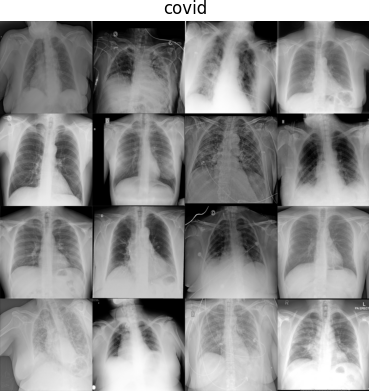
\includegraphics[width=132px]{covid0.png}
    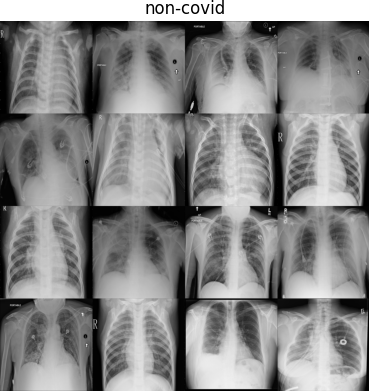
\includegraphics[width=132px]{covid1.png}
    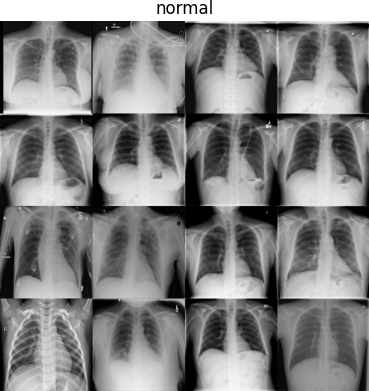
\includegraphics[width=132px]{covid2.png}
    \caption{COVID dataset samples divided by class.}
    \label{fig:covid_dataset}
\end{figure}
\paragraph{Description}
The COVID-QU-Ex dataset \citep{covid} consists of 33,920 chest X-ray (CXR) images including
11,956 COVID-19 images,
11,263 non-COVID infections (Viral or Bacterial Pneumonia) and
10,701 healthy chest X-rays.
It can be found at \url{https://www.kaggle.com/datasets/anasmohammedtahir/covidqu}.
Samples can be seen in Figure \ref{fig:covid_dataset}.
\paragraph{Training}
20\% of the dataset was used as the test set (as proposed by the dataset authors).
Using the VGG16 we obtained 98\% ROC AUC on the test set (mean from the AUC for those three classes).
With ResNet50 we obtained 94\% ROC AUC.

\subsection{Melanoma}
\begin{figure}[t]
    \centering
    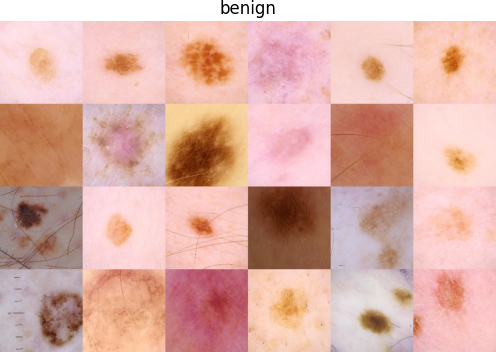
\includegraphics[width=200px]{melanoma0.png}
    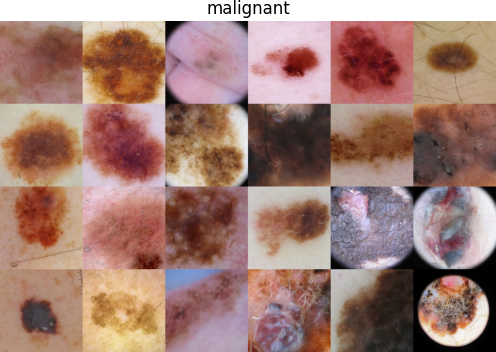
\includegraphics[width=200px]{melanoma1.png}
    \caption{Melanoma dataset samples divided by class.}
    \label{fig:melanoma_dataset}
\end{figure}
\paragraph{Description}
The Melanoma dataset \citep{melanoma} consists of 37,648 dermoscopic training images of unique benign and malignant skin lesions (5,106 malignant and 32,542 benign samples).
It can be found at \url{https://www.kaggle.com/datasets/nroman/melanoma-external-malignant-256}.
Samples can be seen in Figure \ref{fig:melanoma_dataset}.
\paragraph{Augmentations}
The first trained networks were mostly focusing on the edges of the image. It turns out that some images from microscopes are circle shaped and have a black background outside the circle. Furthermore, this property is not balanced between the positives and negatives. We have decided to include an augmentation that simulates that black background from microscopes, which resolved this bias. The final augmentations consist of Color Jitter, Random Perspective, Random Erasing, Random Rotation, and Microscope Simulation (as described above).
\paragraph{Training}
33\% of the dataset was used as the test set.
Using the VGG16 we have managed to obtain 94\% ROC AUC on the test set.
Using ResNet50 we obtained 93\% ROC AUC.

\section{Enhanced LRP visualizations} \label{appendix:lrp}
In this appendix, we present results for the LRP method with different composites (Figure \ref{fig:lrp_long} and Figure \ref{fig:lrp_tta_long}).
We found out that EpsilonPlusFlat works best so in the main report we only focus on the mentioned composite.

\begin{figure}[t]
    \centering
    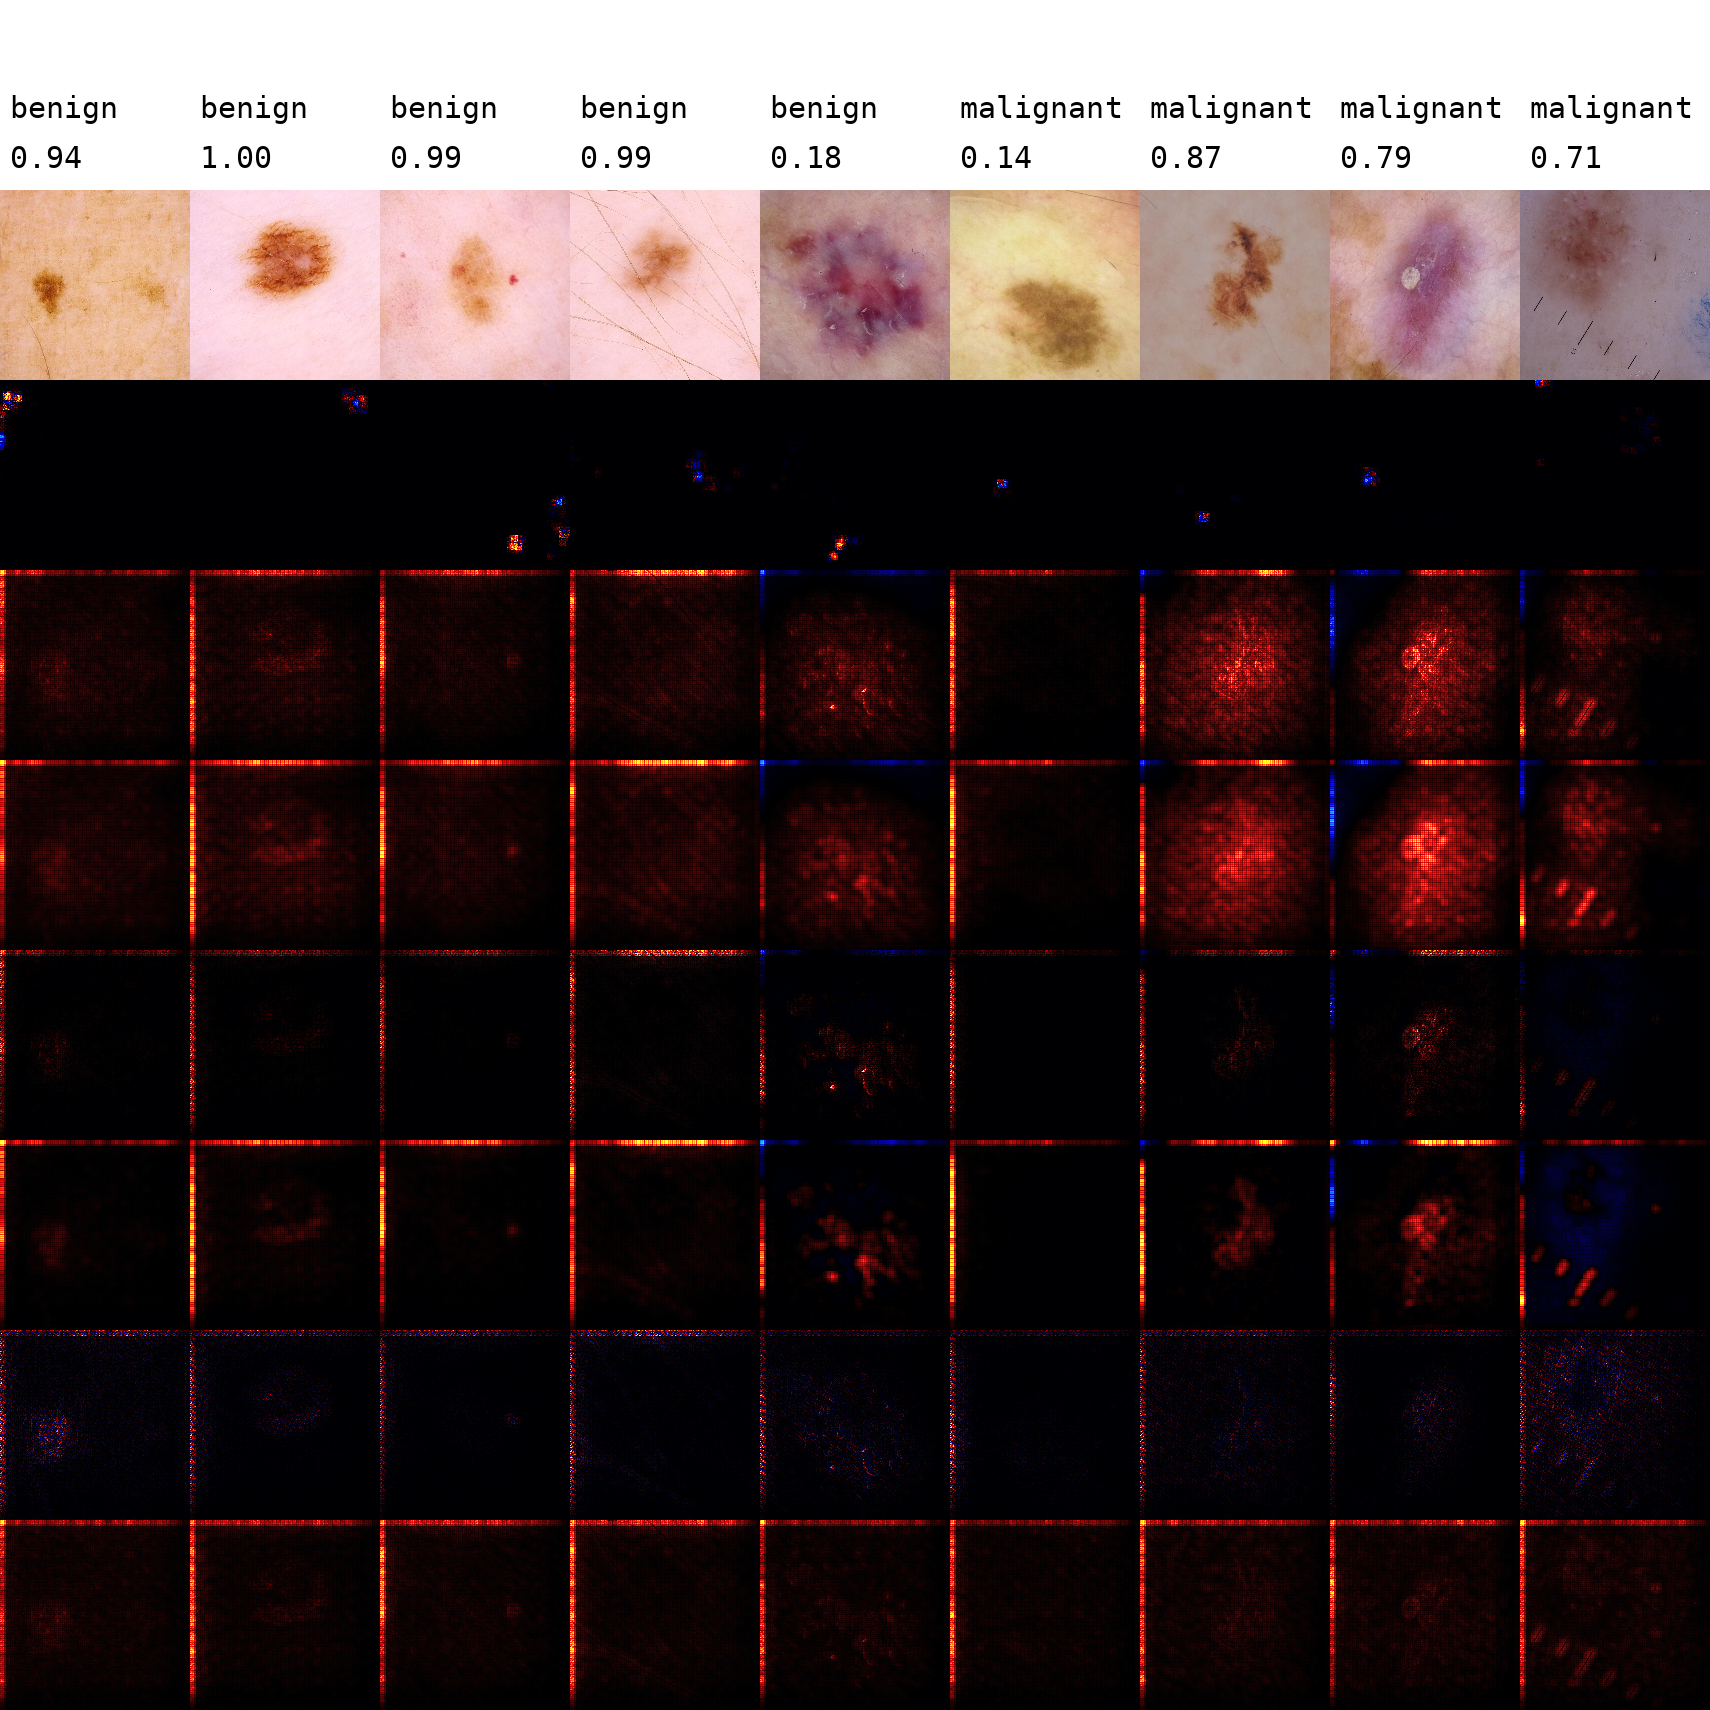
\includegraphics[width=200px]{melanoma_resnet.png}
    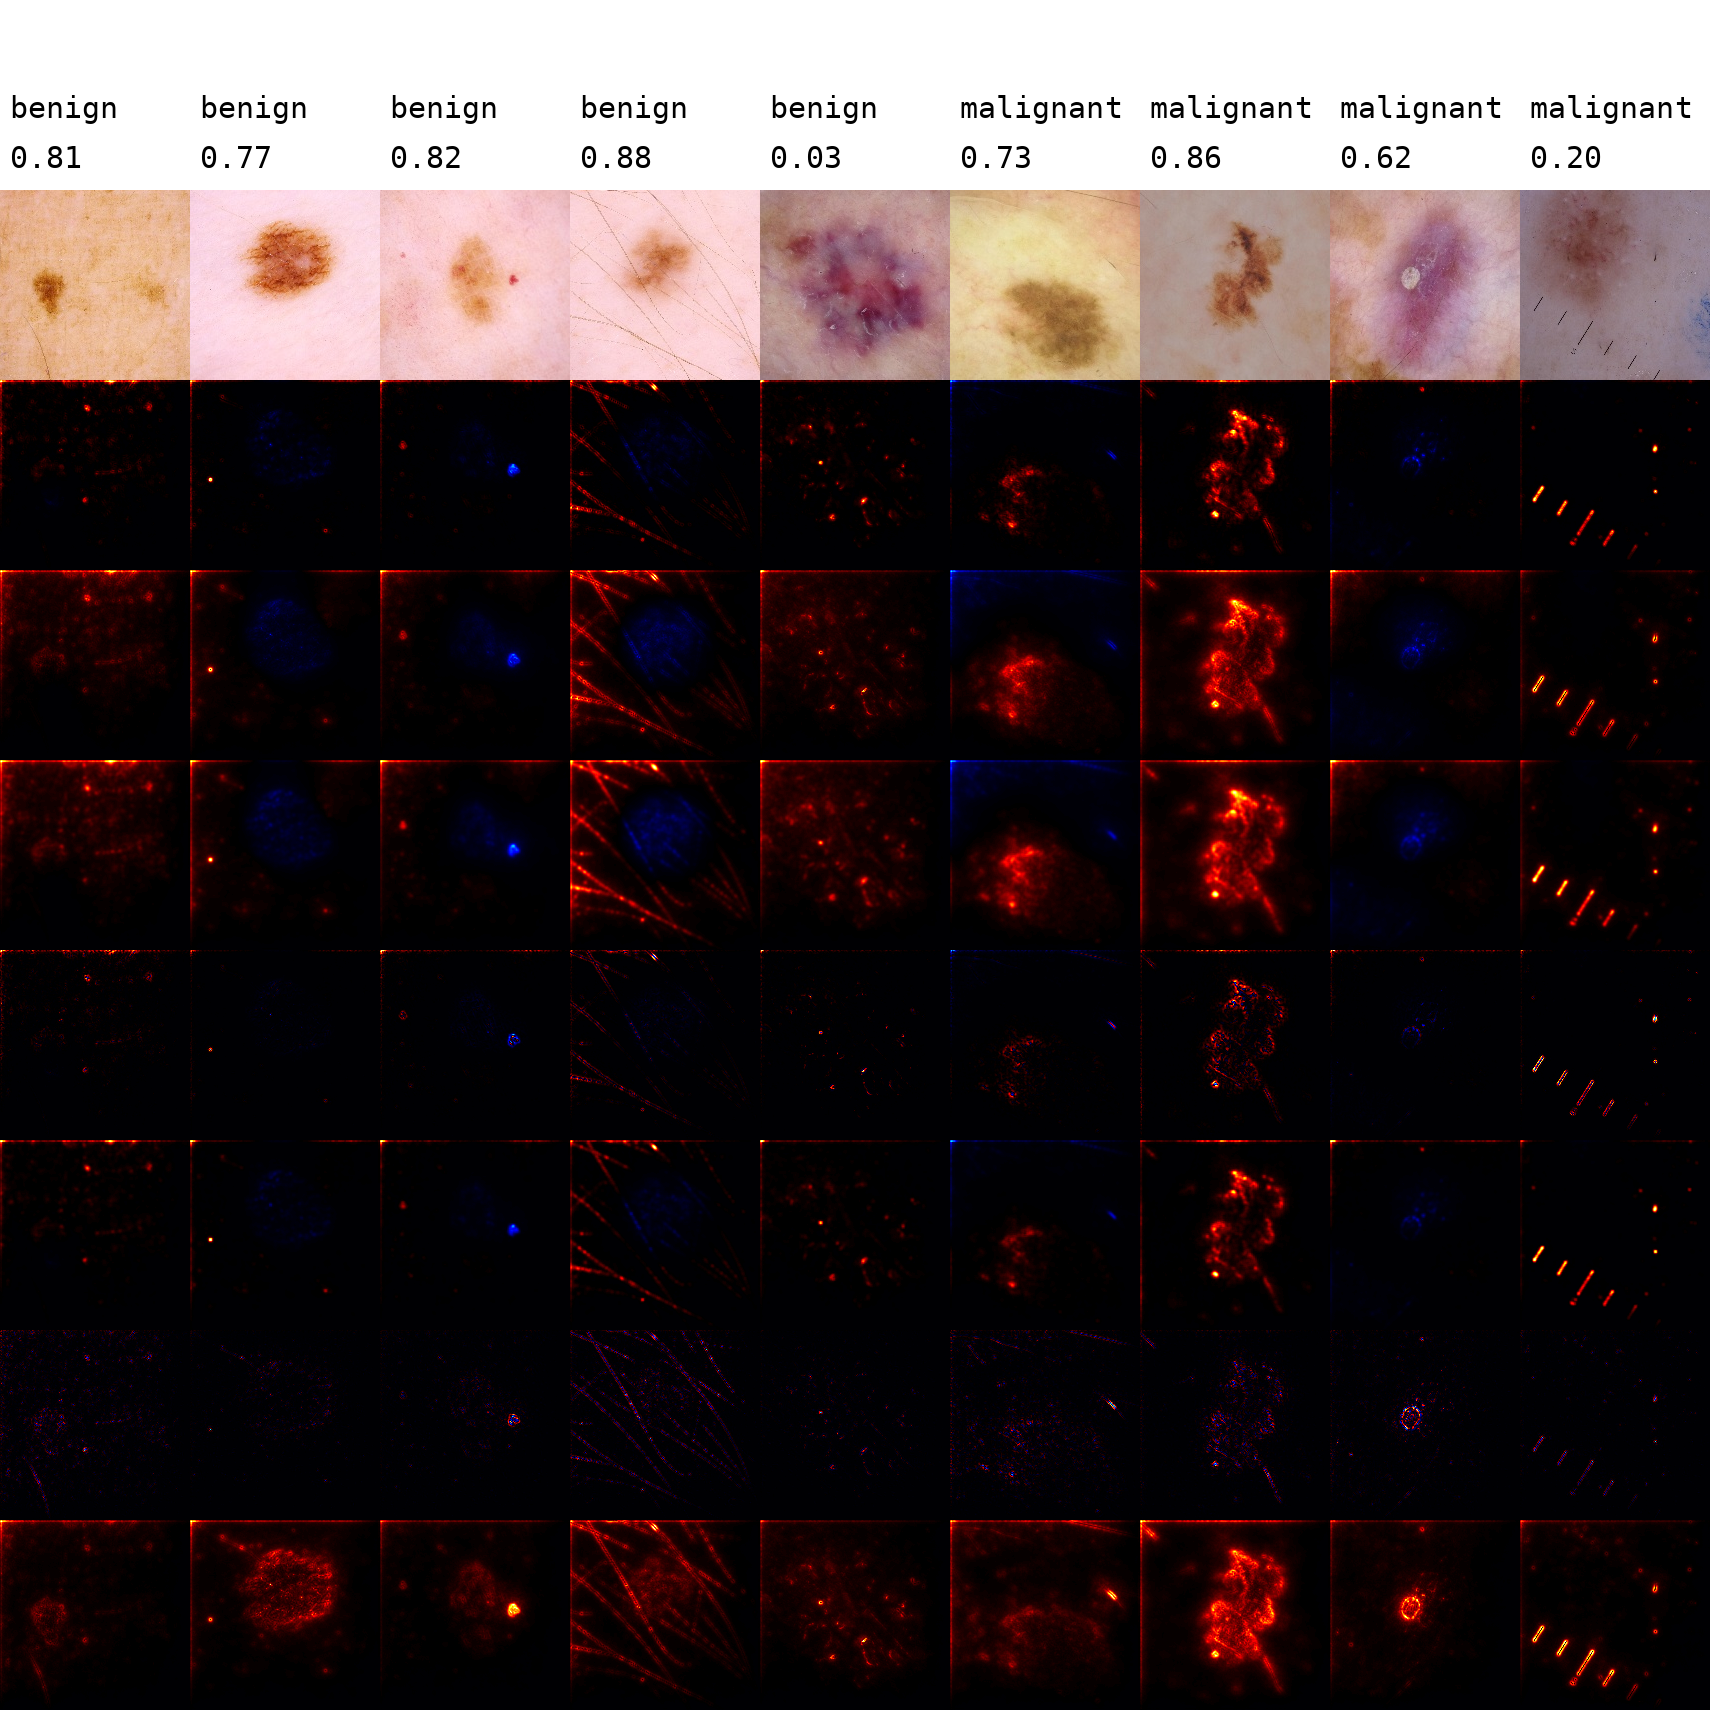
\includegraphics[width=200px]{melanoma_vgg.png}
    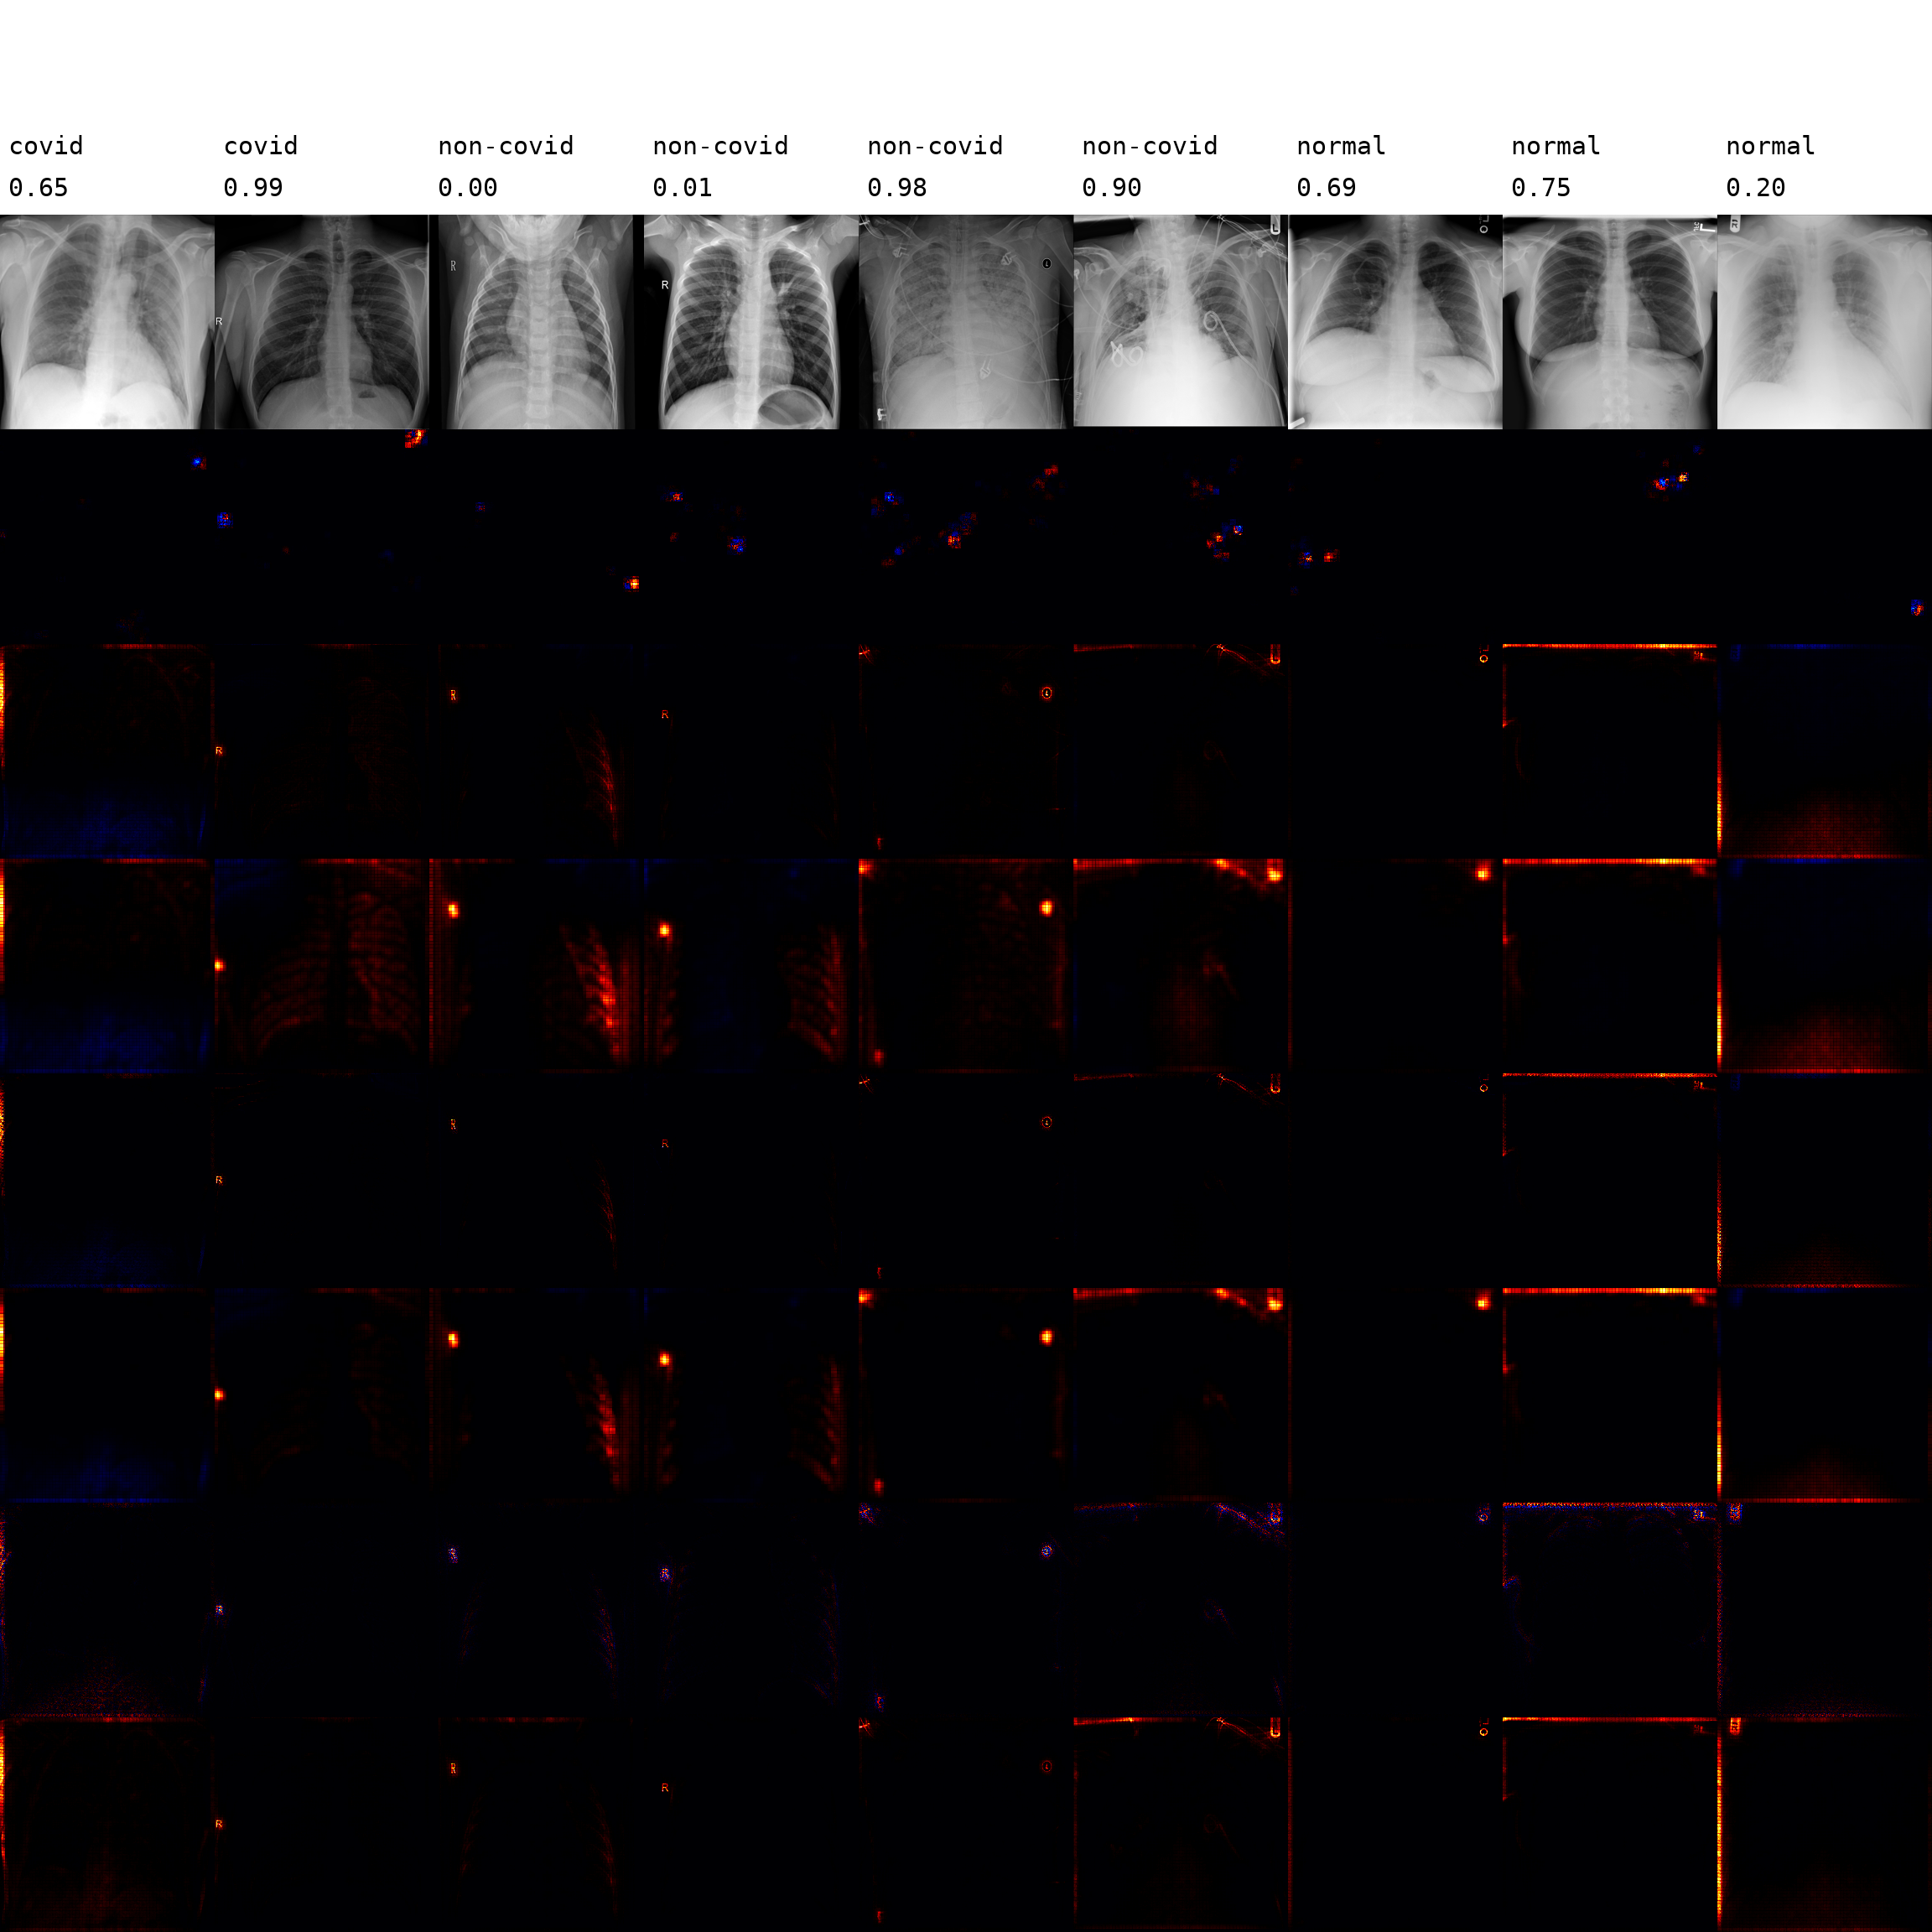
\includegraphics[width=200px]{covid_resnet.png}
    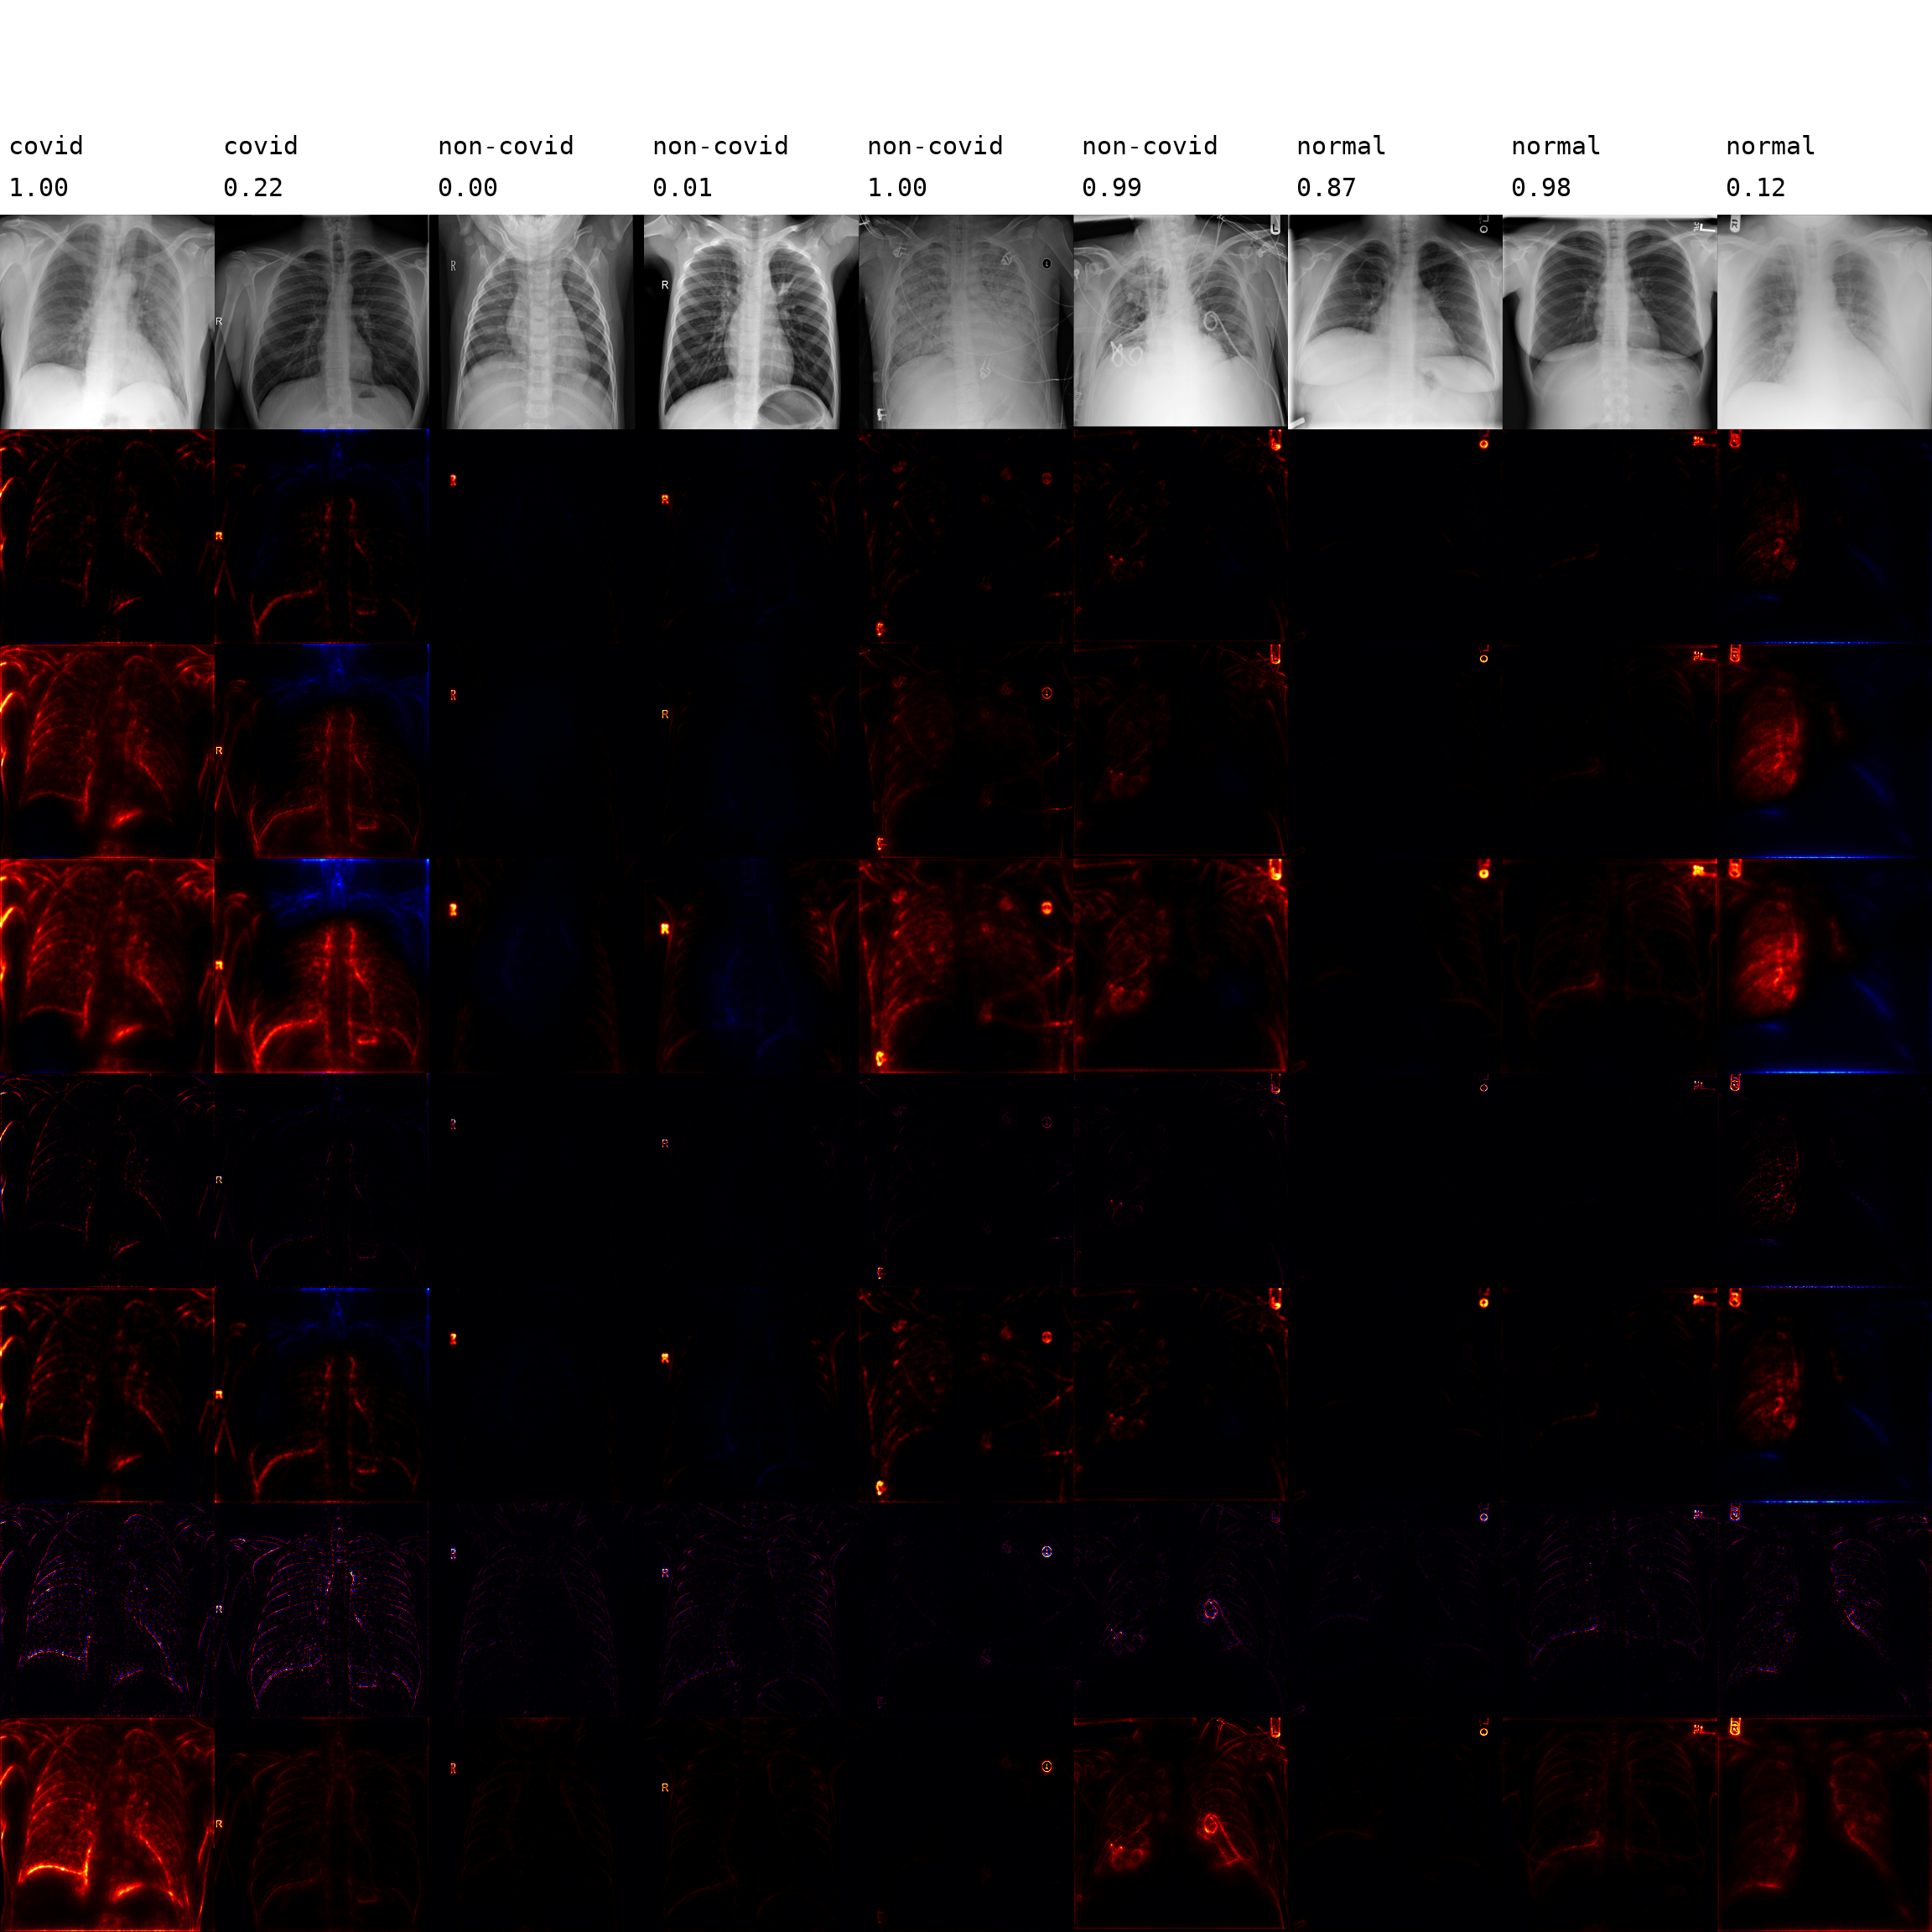
\includegraphics[width=200px]{covid_vgg.png}
    \caption{
    Melanoma LRP results (top left: ResNet50, top right: VGG16) and COVID LRP results (bottom left: ResNet50, bottom right: VGG16).
    On each image the rows are: class name, prediction on the class, input image, LRP explanations with composite: EpsilonGammaBox, EpsilonPlus, EpsilonPlusFlat, EpsilonAlpha2Beta1, EpsilonAlpha2Beta1Flat, GuidedBackprop, ExcitationBackprop.
    }
    \label{fig:lrp_long}
\end{figure}
\begin{figure}[t]
    \centering
    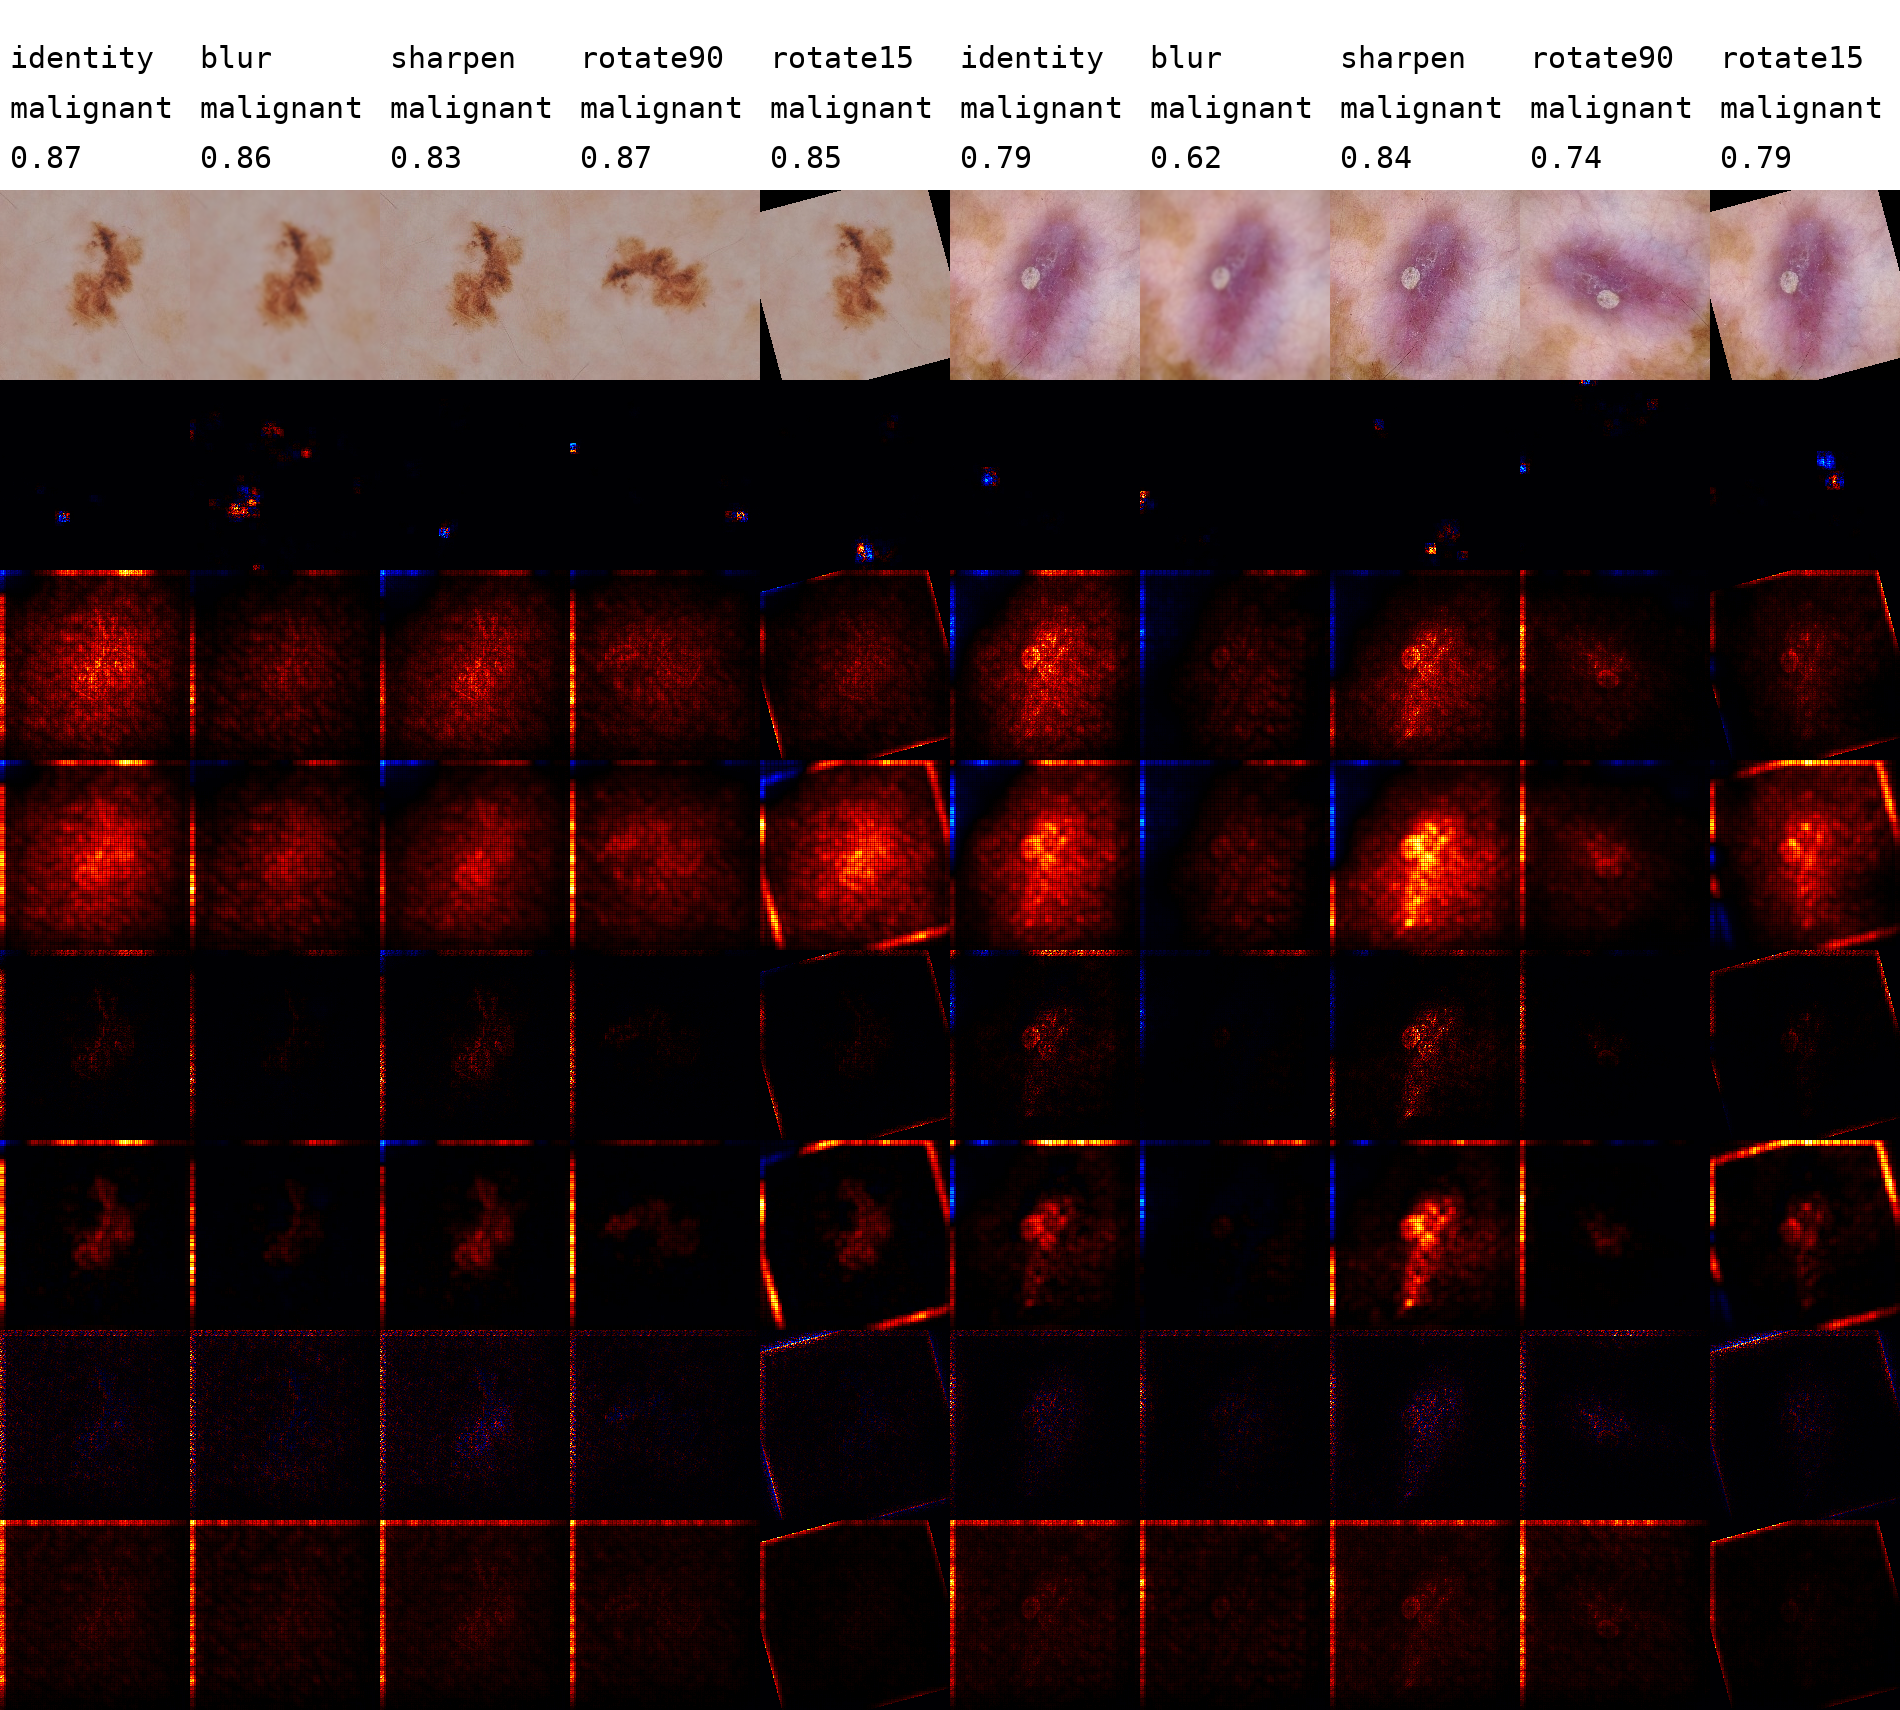
\includegraphics[width=200px]{tta_melanoma_resnet.png}
    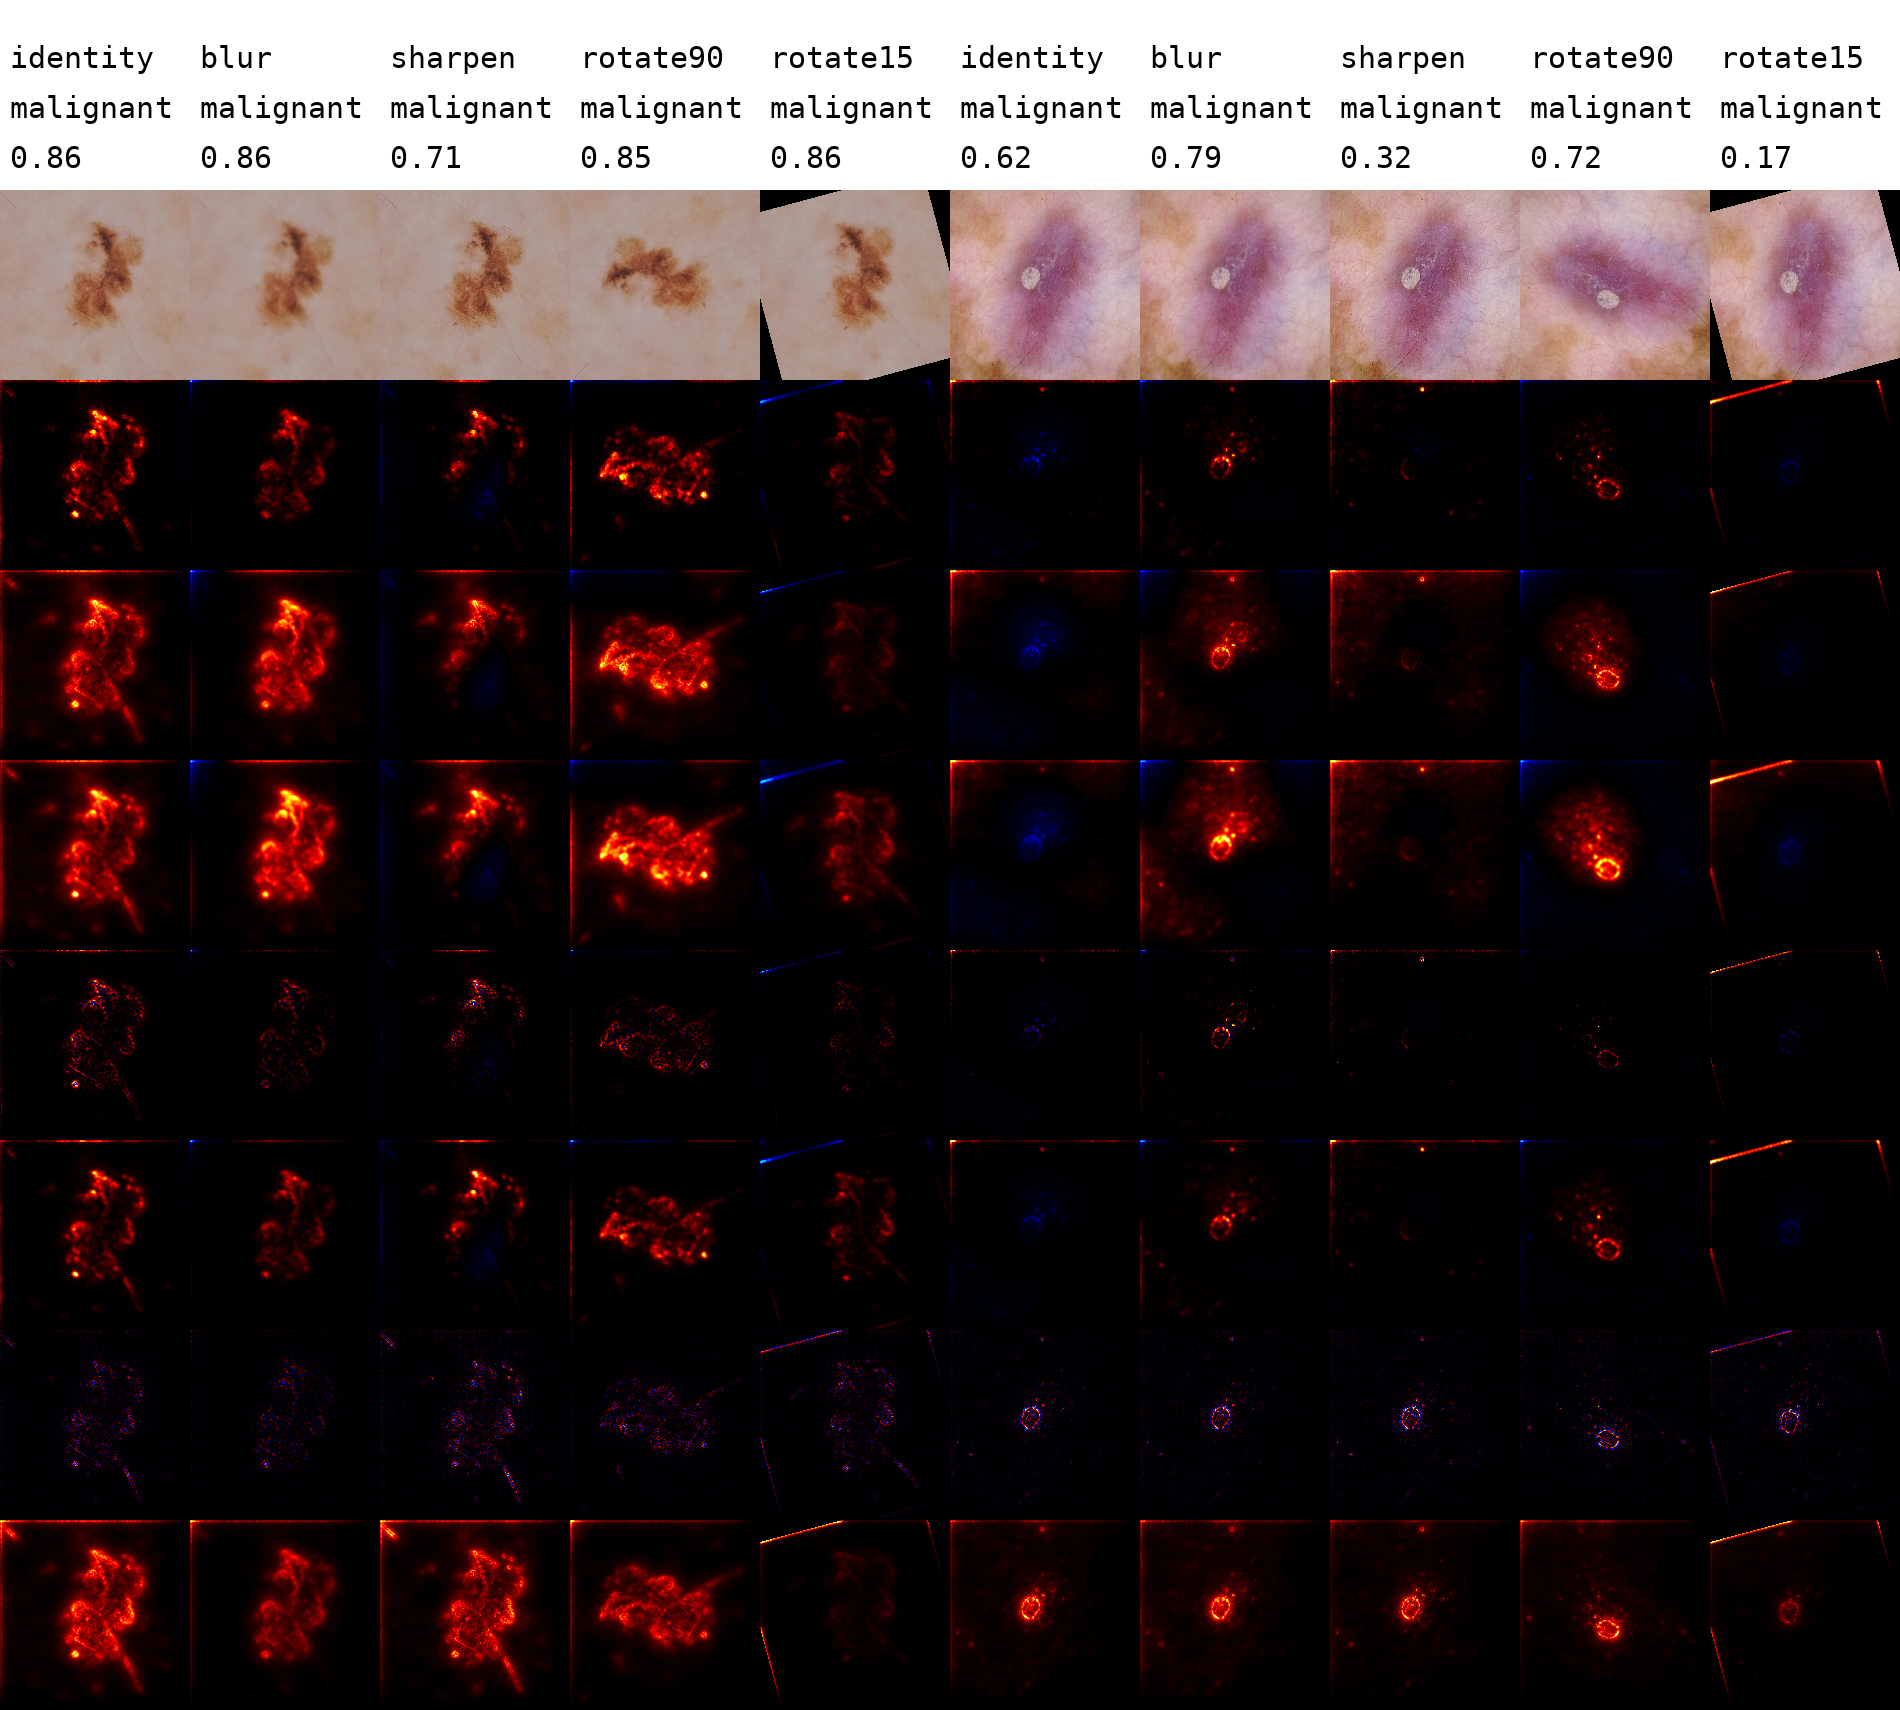
\includegraphics[width=200px]{tta_melanoma_vgg.png}
    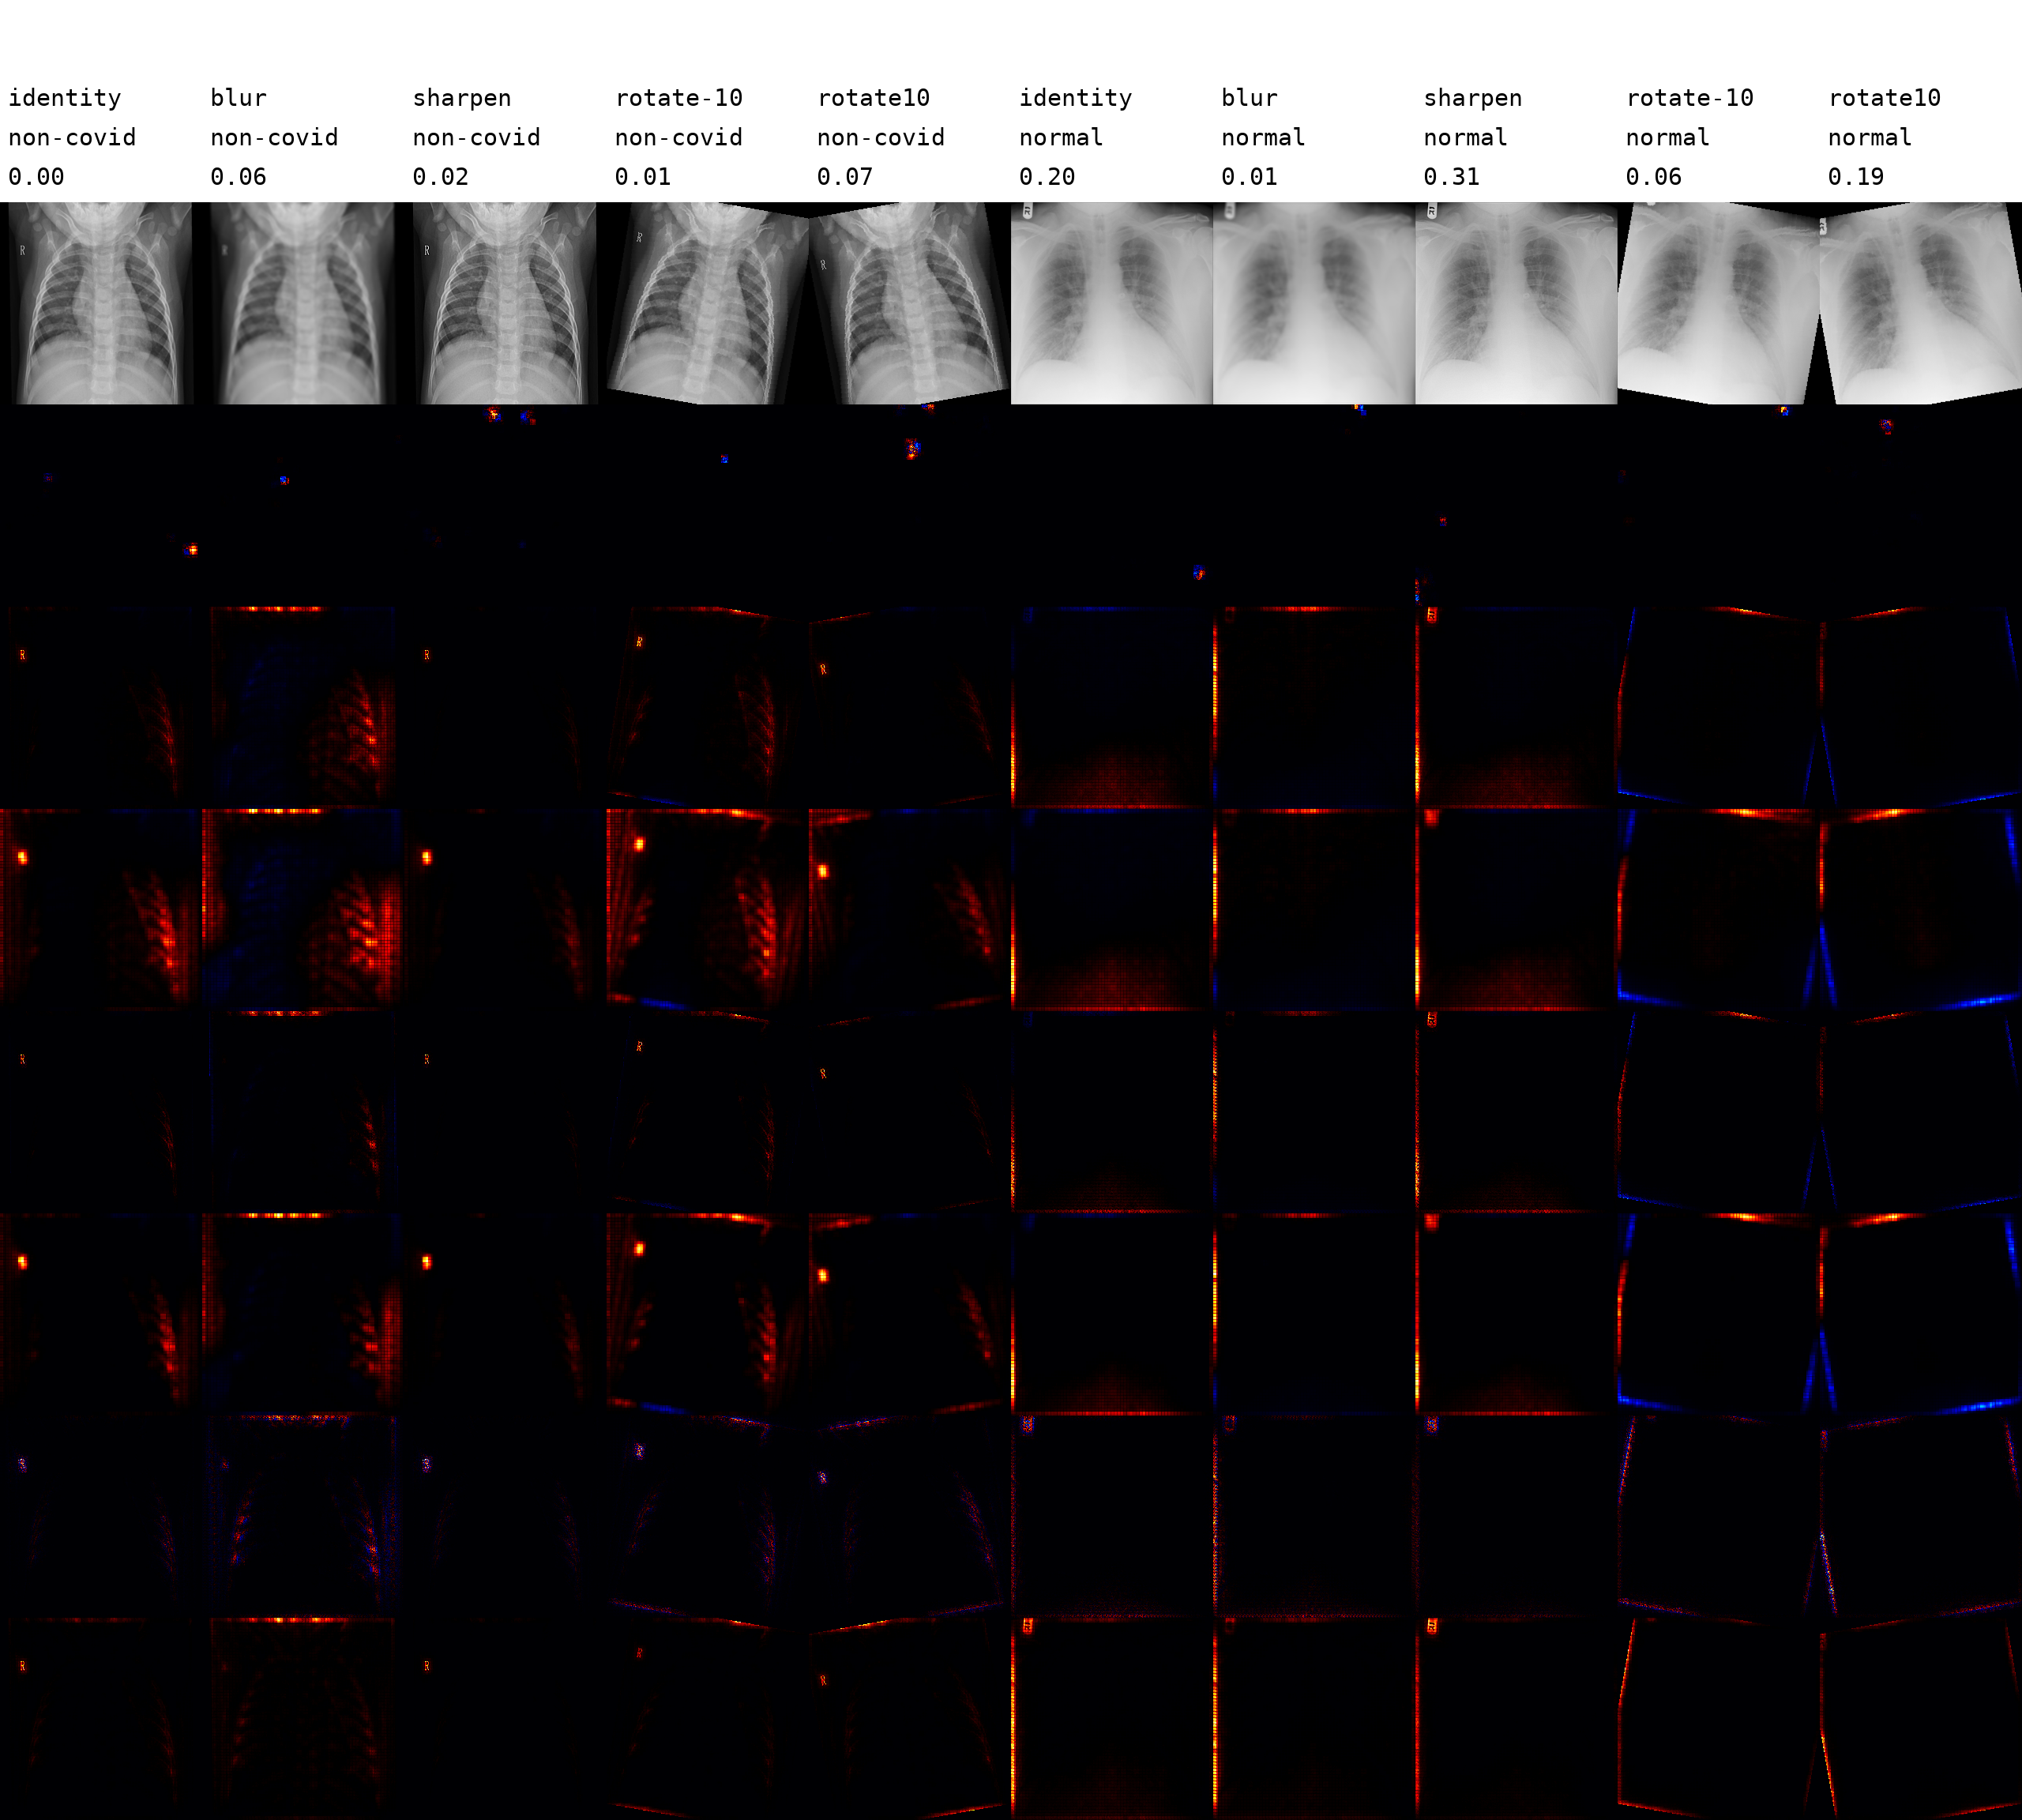
\includegraphics[width=200px]{tta_covid_resnet.png}
    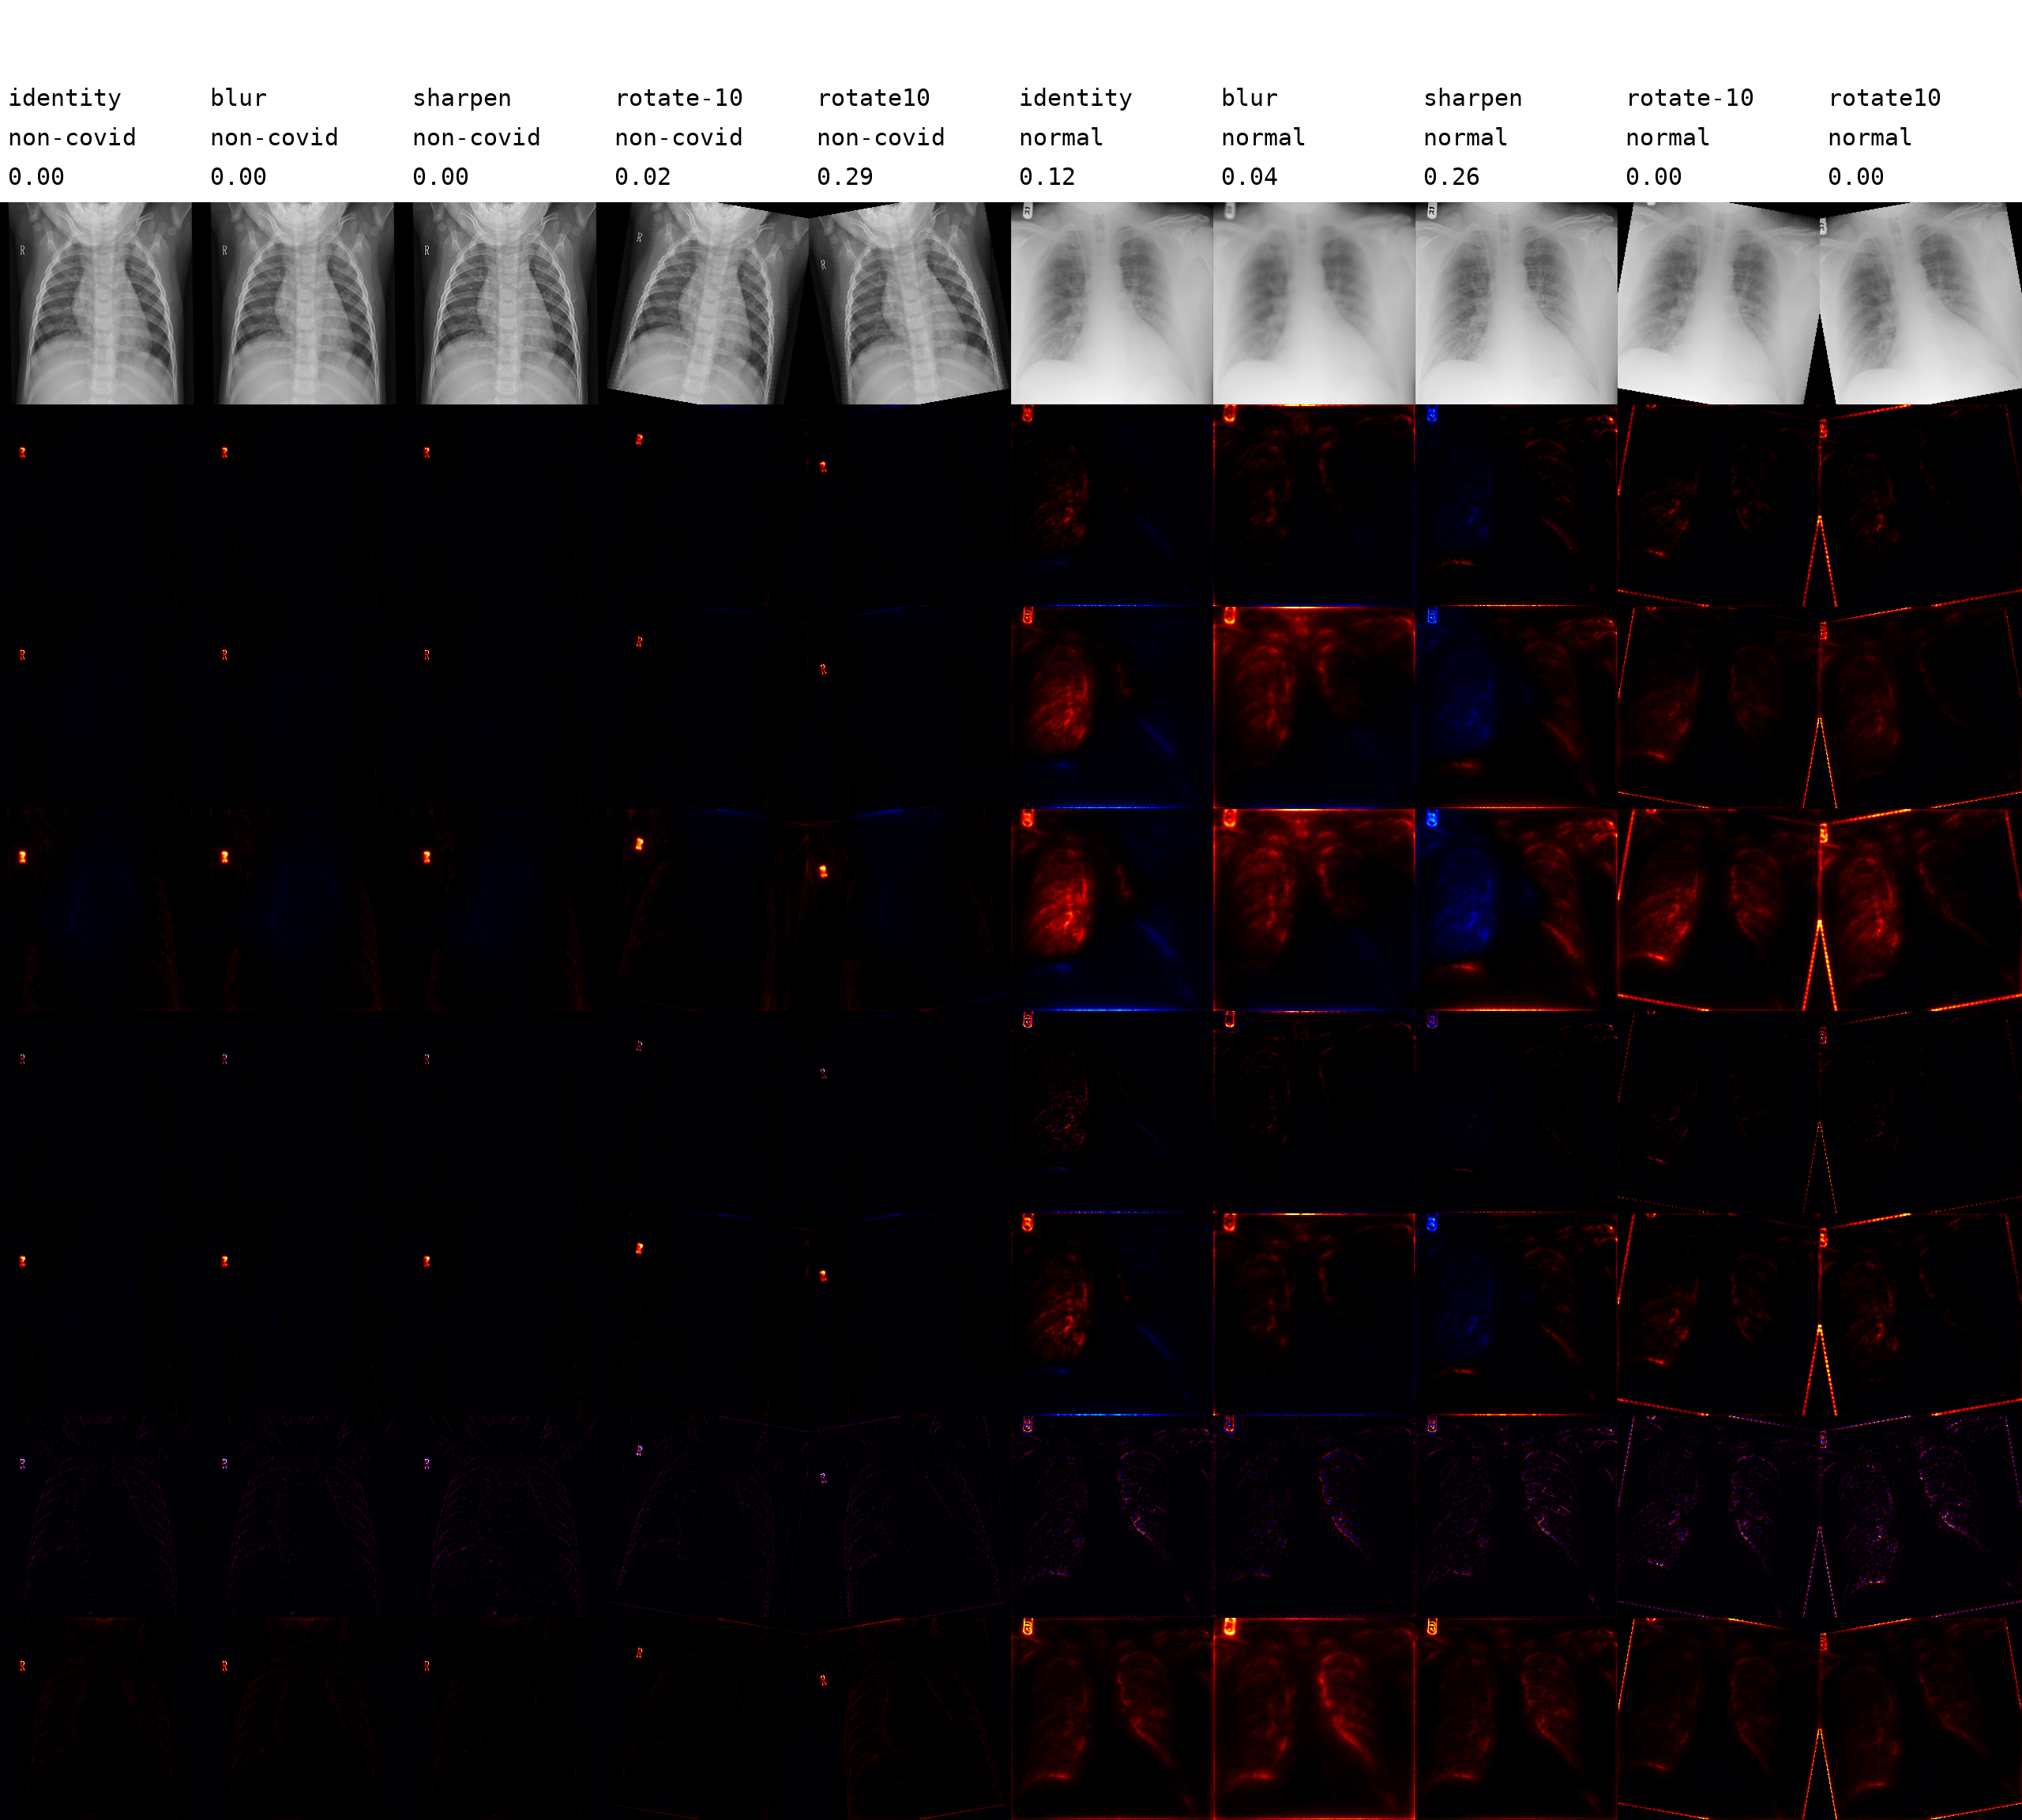
\includegraphics[width=200px]{tta_covid_vgg.png}
    \caption{
    Results for LRP after input augmentation.
    Melanoma LRP results (top left: ResNet50, top right: VGG16) and COVID LRP results (bottom left: ResNet50, bottom right: VGG16).
    On each image the rows are: augmentation name, class name, prediction on the class, input image, LRP explainations with composite: EpsilonGammaBox, EpsilonPlus, EpsilonPlusFlat, EpsilonAlpha2Beta1, EpsilonAlpha2Beta1Flat, GuidedBackprop, ExcitationBackprop.
    }
    \label{fig:lrp_tta_long}
\end{figure}

\section{CRP experimental setup} \label{appendix:crp_setup}
The setup we followed for interpreting the model's prediction using the CRP method is that we looked at conditioning on each layer, using the concept that was ranked as the most relevant for the prediction. In this report, we only show the most interesting features found for each dataset and model. We look at the same datasets and models as in the case of the LRP method. It was not trivial to apply CRP to ResNet since the residual connections caused the relevance to pass despite the masks being present. We were able to solve it by calculating the attributions twice, once conditioned on the concept we wanted, and once conditioned on a layer with no concepts, which allowed us to get exactly the relevance that was passed there through the residual connections.
\end{document}
